%!TEX root = ../dissertation.tex
\begin{savequote}[75mm]
In theory, theory and practice are the same thing, but in practice...
\qauthor{Adam Savage}
\end{savequote}

\chapter{Johnson noise thermometry}
\label{ch:johnson_noise_thermometry}

\newthought{Given any process in which an applied force generates heat}, the reverse process must also exist and, therefore, thermal fluctuations must cause fluctuations in that force. The idea that the same physics governing the dissipation of a object moving through some environment is responsible for the apparent random motion of that object was originally described by Einstein in the context of pollen grains ~\cite{einstein_investigations_1956}. The generalized fluctuation-dissipation theorem~\cite{kubo_fluctuation-dissipation_1966} quantifies this statement for linear systems\footnote{Here a linear system is one where the force acting on a particle is proportional to its velocity --- i.e.$F/v$ is constant} by relating the power spectral density $S_P(\omega)$ to the real part of the generalized impedance $Z(\omega)$~\cite{callen_irreversibility_1951}.
\begin{equation}\label{eq:fluctuation_dissipation}
S_P(\omega) \propto k_BT\ \Re[Z(\omega)]
\end{equation}
Nearly a quarter of a century later, Nyquist~\cite{nyquist_thermal_1928} related Einstein's description of Brownian motion to the electrical noise measured by Johnson~\cite{johnson_thermal_1927,johnson_thermal_1928}. Although all the key components were in place, it would take until 1946 for the first noise thermometer to be built~\cite{dicke_measurement_1946}. The general idea is to measure the noise spectrum emitted by a device and thus determine its electronic temperature. Johnson noise thermometry (JNT) is analogous to radiation thermometry where the blackbody spectrum of an object is used to determine its temperature --- in fact, both rely upon modified versions of eq~\ref{eq:fluctuation_dissipation}

\section{Thermal noise in resistors}
Johnson noise, often referred to as Johnson-Nyquist noise, was first measured in 1927~\cite{johnson_thermal_1927}. Johnson found the fluctuations in the squared voltage across a resistor were linearly proportional to both the resistance and the temperature and independent of the conductor being measured. The following year, Nyquist derived the form of the noise spectral density from thermodynamic arguments; consider two identical resistors in thermal equilibrium at a temperature T connected such that any noise emitted by one is absorbed by the other, as shown in Fig.~\ref{fig:Nyquist_resistors}. As we are in thermal equilibrium, we know the power being absorbed by a given resistor per unit frequency must be equal to the thermal energy being emitted, $k_BT$. If we represent the Johnson noise of the first resistor as a series voltage source with squared fluctuations, $V_{JN}$, the power dissipated in the second resistor per unit frequency is given by $I^2R = V_{JN}^2 / 4R$ as the total resistance of the circuit is $2R$. Setting this equal to $k_BT / \Delta f$ leads us to Nyquist's famous result.
\begin{equation}\label{eq:Nyquist}
S_{V}(\omega) = 4Rk_BT
\end{equation}
\begin{figure}
\centering
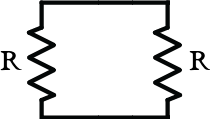
\includegraphics[height = 25mm]{figures/Johnson_noise_thermometry/Nyquist_resistors.png}
\caption{Schematic of Nyquist's famous thought experiment. Two resistors in thermal equilibrium are connected end to end and allowed to transfer energy between them via thermal current fluctuations.}
\label{fig:Nyquist_resistors}
\end{figure}
This derivation holds regardless of the conductor, be it an electrolytic solution or graphene in a quantum Hall state. However, there is a glaring problem with extending this formula to high frequency; similar to the UV-catastrophe in black-body radiation, Nyquist's formula extends to infinite energies as it lacks a high frequency cutoff. This is fixed by quantum mechanics resulting in a rolloff of the noise spectrum centered at $\hbar\omega = k_BT$.
\begin{equation}\label{eq:NyquistFull}
S_V(\omega) = 4\hbar\omega~\Re(Z)\left[\frac{1}{2}+\frac{1}{exp(\hbar\omega/k_BT)-1}\right]
\end{equation}
This high frequency cutoff was seen experimentally by Schoelkopf, et al.~\cite{schoelkopf_frequency_1997} and is only of practical import at high frequencies ($>1~GHz$) and low temperatures ($<1~K$).

\section{Resistor networks: The Johnson noise temperature}
\label{section:TJN}
\newthought{As noise is a random process}, adding multiple resistors together into a network is not a simple matter of adding their voltages and/or currents but instead their mean squared voltages $\langle V^2\rangle$ and/or mean squared current $\langle I^2\rangle$. This is a property of Gaussian distributed noise: adding together two Gaussian distributions, each with mean $0$ and variance $\sigma$, with result in another Gaussian distribution with mean $0$ and variance $2\sigma$\footnote{This is why mean squared error is often a useful metric. If errors are unbiased and Gaussian distributed then summing their variance is appropriate}.

To find the noise emitted by two resistors in series with resistance $R_1$ and $R_2$ and temperature $T_1$ and $T_2$, we add their mean squared voltages.
\begin{equation} \label{eq:seriesJN}
\langle V^2\rangle = 4k_B (R_1T_1+R_2T_2)\Delta f
\end{equation}
While in the case of the same two resistors in parallel we must add their mean squared currents.
\begin{equation} \label{eq:parallelJN}
\langle I^2\rangle = 4k_B \left(\frac{T_1}{R_1}+\frac{T_2}{R_2}\right)\Delta f
\end{equation}
This process can be extended to any network of discrete, two-terminal resistors.

An effective ``Johnson noise temperature" for a given resistor network can be defined as the temperature, $T_{JN}$, such that the total noise emitted between two given terminals of the network is:
\begin{equation}
\langle V^2\rangle = 4k_BR\Delta f * T_{JN}
\end{equation}
where $R$ is the two-terminal resistance. For an arbitrary network with many terminals, $T_{JN}$ will differ depending upon which two-terminals the noise is measured between. For resistors in series we can see from Eqn.~\ref{eq:seriesJN}
\begin{equation}
\langle V^2\rangle = 4k_BR \left(\frac{R_1}{R}T_1+\frac{R_2}{R}T_2\right)\Delta f
\end{equation}
and thus we can define the Johnson noise temperature for this network as:
\begin{equation}
T_{JN}^{\ series} = \sum_i \frac{R_i}{R}T_i
\end{equation}
Similarly from Eqn.\ref{eq:parallelJN} we see that for resistors in parallel
\begin{equation}
\langle V^2\rangle = \langle I^2\rangle\times R^2 = 4k_BR\Delta f (\frac{R}{R_1}T_1+\frac{R}{R_2}T_2)
\end{equation}
\begin{equation}
T_{JN}^{\ parallel} = \sum_i \frac{R}{R_i}T_i
\end{equation}

These equations are unified by considering the relationship between the power dissipated in a particular resistor $P_i$ from a voltage across the two terminals of the network (or equally a current across the network) compared to the total power dissipated over the entire network $P_0$. For the resistors in series $P_i/P_0 = R_i/R$ and for resistors in parallel $P_i/P_0 = R/R_i$. Thus in both cases:
\begin{equation}\label{eq:TJN_discrete}
T_{JN} = \sum_i\frac{P_i}{P_0}T_i
\end{equation}
In fact this is quite general and holds for any combination of resistive elements. It stems from the fluctuation dissipation theorem and can be summarized by the statement: The voltage fluctuations created between two terminals of a resistor network due to the thermal fluctuations of a given element in that network are exactly given by the power dissipated in that element due to an external voltage placed on those terminals.

In the continuous limit, Eqn.~\ref{eq:TJN_discrete} can be used to find the noise emitted by a device with a spatially non-uniform temperature profile $T(\vec{r})$ by solving for the spatial power dissipation profile $\mathcal{P}(\vec{r})$.
\begin{equation}\label{eq:TJN_cont}
T_{JN} = \frac{\int \mathcal{P}(\vec{r})*T(\vec{r}) d\vec{r}}{\int \mathcal{P}(\vec{r}) d\vec{r}}
\end{equation}
where $\vec{r}$ is over the spatial dimensions of the device. Eqn.~\ref{eq:TJN_cont} is the main result of this section.


\section{Johnson noise in RF circuits}
\newthought{When measuring Johnson noise at high frequency}, it can be useful to reformulate the problem into the language of microwave circuits. The Nyquist theorem, Eqn.~\ref{eq:Nyquist}, can be rewritten to describe the average power, $\langle\mathrm{P}\rangle$, absorbed by an amplifier coupled to a device with reflection coefficient $\Gamma^2$:
\begin{equation}\label{eq:NyquistPower}
\langle\mathrm{P}\rangle = k_BT\Delta f~~(1-\Gamma^2)
\end{equation}
and
\begin{equation}\label{eq:Gamma}
\Gamma = \frac{Z-Z_0}{Z+Z_0}
\end{equation}
where $Z$ is the complex impedance of the device and $Z_0$ is the impedance of the measurement circuit --- typically $50~\Omega$. In this form is it quite easy to see the thermodynamic origins of the Nyquist equation. A device at temperature $T$ radiates a power of $k_BT$ per unit frequency; some of that power is absorbed by the measurement circuit, and some is reflected back to the sample. All the resistance dependence of the noise power is captured by $\Gamma$\footnote{this is also a nice proof for why $\Gamma$ in any non absorptive 2 port device must be symmetric, $\Gamma_{12}=\Gamma_{21}$. If this was not true, we could place the device between two resistors in thermal equilibrium and one would heat the other. Two-port devices which report asymmetric coefficients often include internally terminated third ports.}.
With this new formulation the importance of minimizing $\Gamma$ become apparent. For effective high frequency Johnson noise thermometry we must match the impedance of the device to the measurement circuit. For devices with two-terminal resistances far from $50~\Omega$, it is beneficial to add impedance matching circuits to transform the device to match $Z_0$ --- in practice resistances less than $\sim 10~\Omega$ or grater than $\sim 250~\Omega$ benefit from matching circuits.
As can be seen from Eqn.~\ref{eq:NyquistPower}, the larger the measurement bandwidth $\Delta f$ the larger noise signal. In practice, measurement bandwidths are often limited by either the impedance matching circuitry or the amplifier bandwidth; operating at higher frequencies increases typically increases both these limiting bandwidths.

\section{An autocorrelation RF noise thermometer}
\label{section:autocorrelation}
\begin{figure}
\centering
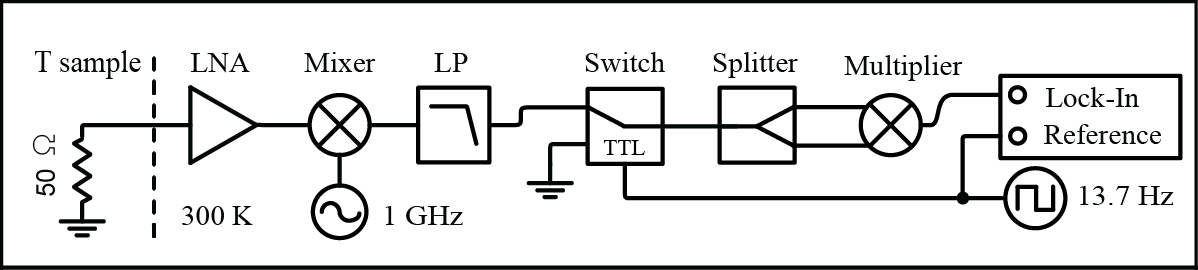
\includegraphics[width=\textwidth]{figures/Johnson_noise_thermometry/Schematic_Autocorrelation.png}
\caption[JNT autocorrelation schematic]{High level schematic of a typical Johnson noise thermometry measurement circuit. Noise from an impedance matched sample is amplified and a measurement bandwidth is selected using a homodyne mixer and low-pass filter. The noise power is then measured with a power diode or linear multiplier. A microwave switch acts as a chopper and the signal is measured using a lock-in amplifier.}
\label{fig:schematic_autocorrelation}
\end{figure}

Fig.~\ref{fig:schematic_autocorrelation} shows an example of a typical, Dicke style~\cite{dicke_measurement_1946}, radiometer used to measure the temperature of a $50~\Omega$ sample. Radiation from the resistor is coupled into a transmission line terminated with a low noise amplifier (LNA). A typical noise spectrum directly from the output of the LNA is shown in Fig.~\ref{fig:Miteq_spec}. The signal-to-noise ratio of a noise measurement is mostly determined the front-end LNA~\cite{pozar_microwave_2011} so care should be taken in selecting the right amplifier. The SiGe LNA (Caltech CITLF3) used throughout the majority of this thesis has a room temperature noise figure, in the frequency range of $0.01$ to $2~GHz$, of about $0.64~dB$, corresponding to an intrinsic noise temperature of 46 K.
\begin{figure}
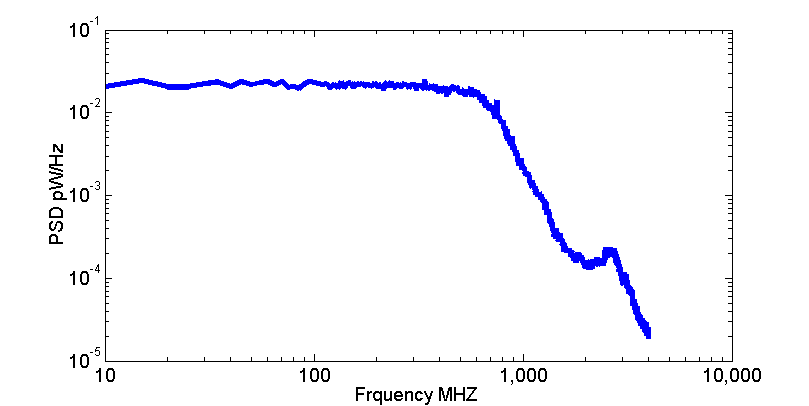
\includegraphics[width=\textwidth]{figures/Johnson_noise_thermometry/Miteq_spec.png}
\caption{a typical spectrum directly from the output of a low noise amplifier (Miteq AU-1291, $\sim$65~dB gain, $\sim$100~K noise temperature) with the input terminated with a 50~$\Omega$ resistor. The spectrum is flat until the amplifier gain begins to roll off above 500~MHz. The amplitude of the ``white" spectrum is proportional to the resistor temperature added to the amplifier noise temperature.}
\label{fig:Miteq_spec}
\end{figure}

Even though Johnson noise has a flat ``white" spectrum, it is important to filter out unwanted $1/f~$ low frequency fluctuations ($\lesssim 10~kHz$) as well as high frequency noise produced where the amplifier gain begins to roll off. 
This can be done using high- and low- pass filters (producing a spectrum similar to that shown in Fig.~\ref{fig:Miteq_BP_spec}, or with a homodyne mixer and low-pass filter combo (as shown in Fig.~\ref{fig:schematic_autocorrelation}. 
\begin{figure}
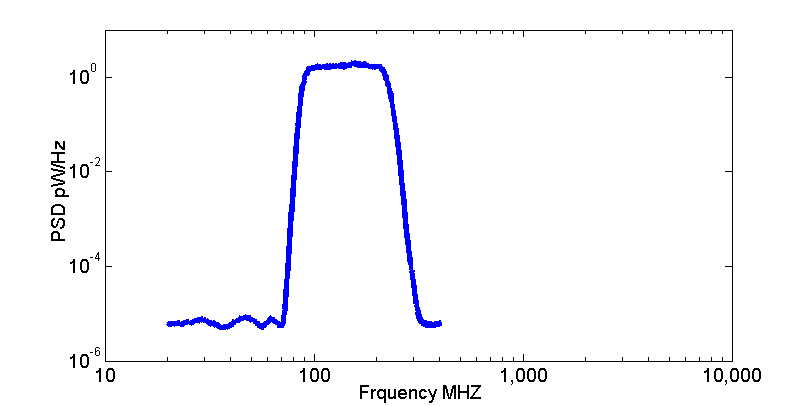
\includegraphics[width=\textwidth]{figures/Johnson_noise_thermometry/Miteq_BP_spec.png}
\caption{a typical Johnson noise spectrum after amplification and filtering using SMA high- and low-pass filters (mini-circuits SLP and SHP series). This square band can then integrated to find the total noise power and thus the temperature of the resistor.}
\label{fig:Miteq_BP_spec}
\end{figure}

Once amplified and cleaned, the total noise power can be measured in a few ways: a spectrum analyzer or digital Fourier transform can read the spectrum directly, a linear multiplier can square the signal and the mean voltage can be measured, or a high frequency power diode and low pass filter combo can convert the power to a proportional DC voltage. Each technique has its own advantages/disadvantages and in a typical experiment multiple techniques are used. 
When presented with a new device or noise setup a spectrum analyzer is often the first measurement to be done; it provides the most in-depth look into the noise of the system and readily shows problem areas such as narrowband noise, parasitic resonances, and/or amplifier performance. After initial setup, however, spectral detail becomes less important and measurements speeds can be significantly enhanced by moving to an all analog setup. 

A linear multiplier (as shown in the schematic Fig.~\ref{fig:schematic_autocorrelation}) can be combined with an RF power splitter and a DC voltmeter to directly measure $\langle V^2\rangle$. Operating from DC to $2~GHz$, the multiplier\footnote{Analog Devices $ADL5931$} serves as a square law detector with 30 dB dynamic range. A JNT using a multiplier is fast and has the added capability of measuring the autocorrelation function, $\langle V(t)V(t-\tau)\rangle$, by simply adding a delay, $\tau$, to one arm of the splitter. While more complicated to setup, once operational a multiplier is a good combination of speed and versatility.

The simplest of the three power detectors discussed here is an RF power diode/low-pass filter combo (e.g. Pasternach PE8000-50). These detectors input an RF signal and output a DC voltage as shown in Fig.~\ref{fig:PE8000}. The output capacitance of these detectors can be quite large so, if a thermal modulation faster than a few 100~Hz is required, care must be taken in choosing an appropriate model. Nevertheless, this is the detector used most commonly in the second half of this thesis due to its wide dynamic range ($30~dB$), small sample package, and ease of use.

\begin{figure}
\centering
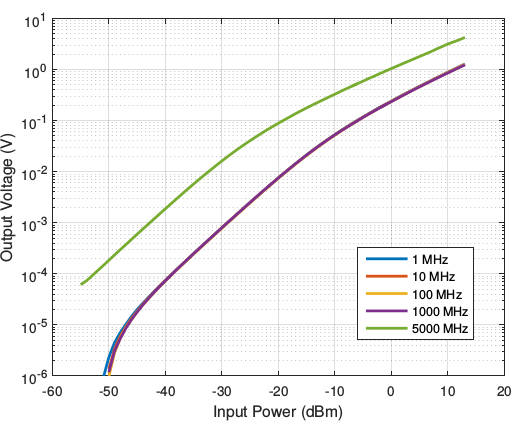
\includegraphics[width = 100mm]{figures/Johnson_noise_thermometry/PE8000-50.png}
\caption{Calibration curves for the Pasternach PE8000-50 power detector. A monochromatic signal of known power is supplied using a microwave source (Stanford Research Systems) and the output is measured using a Voltmeter (Keithley 2400). The detector has a flat frequency response up to 1~GHz and shows linear behavior from -45~dBm to -25~dBm (30~dB dynamic range)}
\label{fig:PE8000}
\end{figure}

Once the noise power is converted to a dc voltage it can be read by a common Voltmeter. To increase the sensitivity it is useful to modulate the noise power. When measuring mesoscopic samples this can be done by modulating the electron temperature via Joule heating. However, in the case of a macroscopic resistor, a microwave switch can be placed after amplification to act as a chopper. The resulting signal can then be measured using a lock-in amplifier.

We can test the noise circuit shown in Fig.~\ref{fig:schematic_autocorrelation} by attaching a resistor to a coldfinger and varying the temperature from $3~K$ to $300~K$. The results are shown in Fig.~\ref{fig:auto_noise_vs_T}. As the sample temperature is lowered, the noise reduces linearly as expected from Eqn.~\ref{eq:NyquistPower}. However, if we extrapolate the data to zero temperature, we see residual noise; this offset is due to all the other (temperature independent) noise sources in the system --- primarily the front-end amplifier. It is useful to quantify this offset in units of Kelvin and is often called the ``system noise temperature". Here we find an system noise temperature of $68~K$ using a room temperature amplifier.
More details on this circuit can be found in Ref.~\cite{crossno_development_2015}

\begin{figure}
\centering
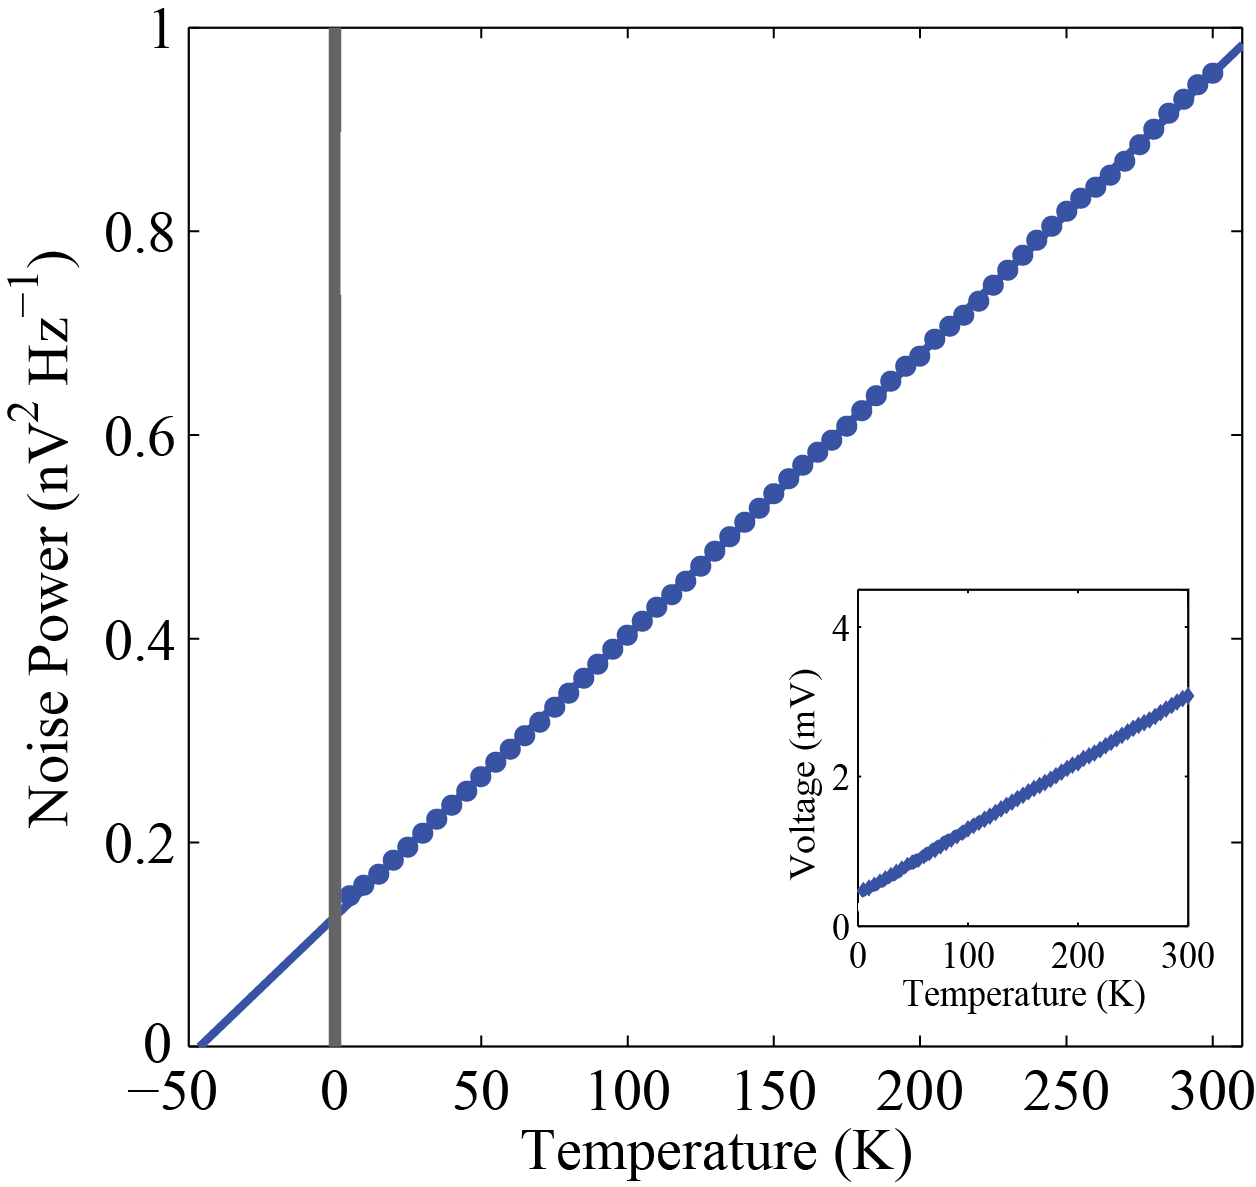
\includegraphics[width = 90mm]{figures/Johnson_noise_thermometry/Auto_noise_vs_T.png}
\caption{Johnson noise of a 50~$\Omega$ resistor measured by the circuit shown in Fig.~\ref{fig:schematic_autocorrelation}. Inset show the lock-in amplifier output. The signal is converted to noise power by the Nyquist equation. The solid line is a linear fit with an offset of 68~K due to amplifier noise}
\label{fig:auto_noise_vs_T}
\end{figure}

\section{Uncertainty in noise measurements}
\newthought{Even noise has noise}. There are $2$ main areas of uncertainty in a noise measurement. The first comes from the fact that noise is stochastic and deals with how well you know the variance of a Gaussian after measuring some amount of time. If the measurements you take are discrete and uncorrelated then we get the usual $1/\sqrt{n}$ dependence, but what do we do if we are measuring a continuous signal? It turns out this is an old problem which stems back to the 1940 and measurements of noise on telephone lines~\cite{rice_mathematical_1944}. In 1944 Rice showed the effective number of uncorrelated measurements is given by the product of the measurement time $\tau$ and the effective noise bandwidth\footnote{The effective noise bandwidth is defined as the width of a perfect square band that passes the same noise power as the true filter function.} $\Delta f$. The surprising fact that the wider the measurement bandwidth the lower the uncertainty, is counter to many experiments where high Q filters are desired to lower the background noise; nevertheless, it can be seen experimentally, as shown in Fig.~\ref{fig:JNT_500measurements}
\begin{figure}
\centering
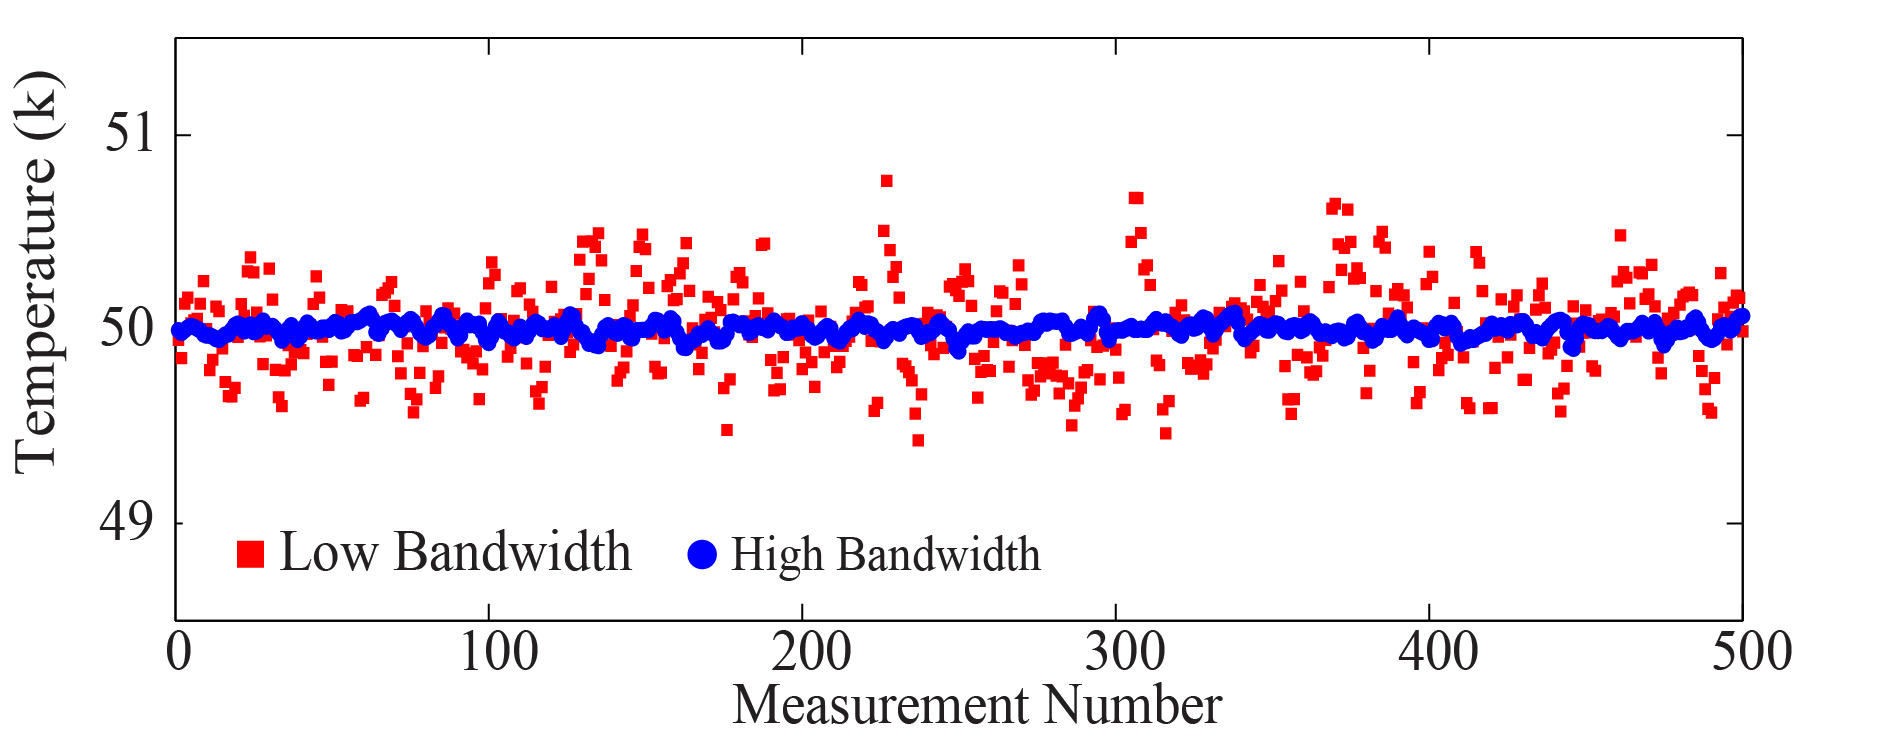
\includegraphics[width=120mm]{figures/Johnson_noise_thermometry/500_measurements.png}
\caption{500 repeated Johnson noise measurements of a $50~\Omega$ resistor at $50~K$ using two different measurement bandwidths. The high bandwidth data has smaller statistical fluctuations than the low bandwidth data.}
\label{fig:JNT_500measurements}
\end{figure}

The second source of uncertainty comes from external noise sources such as amplifiers and boils down to the question: of the noise you measure, what amount comes from the sample? Quantitatively, this can be thought of as a constant offset to the sample temperature and is called the system noise temperature $T_n$\footnote{It should be noted that the system noise temperature can be quite different from an amplifiers intrinsic noise temperature which often assumes a perfectly matched input impedance. See the section~\ref{section:system_noise_temperature} for more details}. In an autocorrelated noise measurement, $T_n$ can be estimated as the offset of a linear fit to the noise power vs sample temperature, as shown in Fig.~\ref{fig:auto_noise_vs_T}. This offset is primarily due to noise in the front-end amplifier but also depends on the sample impedance matching and the bandwidth being measured, as discussed in section~\ref{section:system_noise_temperature}.

Combining these two sources of error we arrive at the famous Dicke radiometer formula~\cite{dicke_measurement_1946}:
\begin{equation}\label{eq:dicke_formula}
\delta T = \frac{T+T_n}{\sqrt{\tau~~\Delta f}}
\end{equation}

We can directly compare Eqn.~\ref{eq:dicke_formula} to experiments by repeating a measurement many times and studying how it fluctuates about the mean. Fig.~\ref{fig:JNT_histograms} compares two histograms, both containing 20,000 autocorrelation measurements at $50~K$ with $50~ms$ integration time but using two different bandwidths: $28$ and $328~MHz$. A sensitivity of $5.5~mK$ $(110 ppm)$ in $1$ second of integration time was achieved using $328~MHz$ bandwidth on a $50~K$ signal.
\begin{figure}
\centering
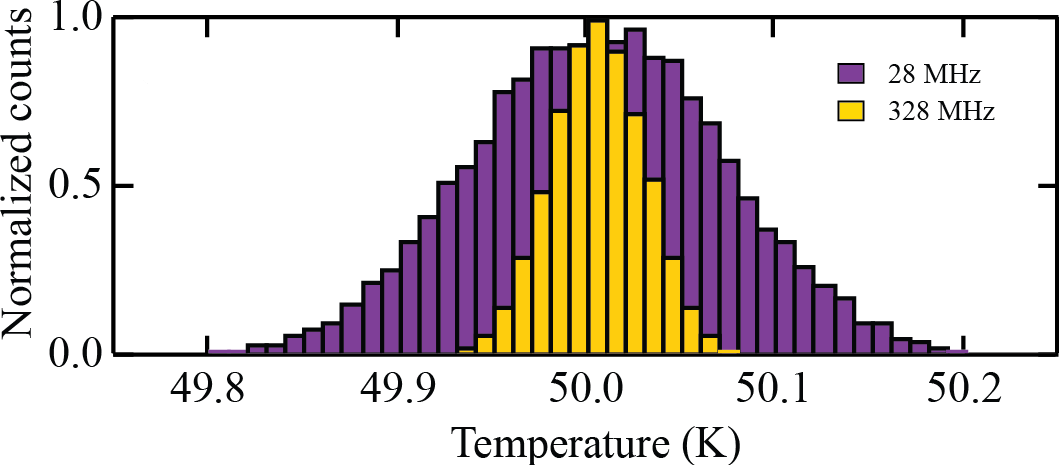
\includegraphics[width = 100mm]{figures/Johnson_noise_thermometry/histograms.png}
\caption{Histograms of 20,000 auto-correlation temperature measurements for $28$ and $328~MHz$ bandwidth using $50~ms$ integration time. Histogram peaks are normalized to 1 for clarity. All data is taken on a $50~K$ resistive load.}
\label{fig:JNT_histograms}
\end{figure}

\section{Impedance matching}\label{section:matching}
\newthought{Life does not always give you $50~\Omega$ samples}. Eqn.~\ref{eq:NyquistPower} illustrates the importance of minimizing the impedance mismatch between the sample and the measurement circuitry -- typically $50~\Omega$. The central principle is to use non-dissipative components to transform the total impedance to $Z(\omega) = 50+0i~\Omega$ at some frequency $\omega = 2\pi\times f$. Impedance matching mesoscopic devices has a unique set of challenges: electrostatic gates and high magnetic fields can cause device impedances to change by multiple orders of magnitude, cryogenic temperatures require the use of only thermally stable components, and large magnetic fields restrict the use of ferrite inductors.

\subsection{LC tank circuits}
\begin{figure}
\centering
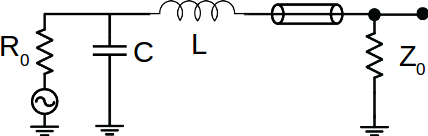
\includegraphics[width=80mm]{figures/Johnson_noise_thermometry/schematic_matching.png}
\caption{Schematic of an LC tank circuit setup in a low-pass configuration used to transform a sample resistance $R_0$ to match the characteristic impedance of a measurement circuit $Z_0$.}
\label{fig:schematic_matching}
\end{figure}
A common way to achieve matching is to use a simple LC circuit. These transformation circuits, known as a tank circuits, can be arranged in several ways but the configuration most useful to these experiments is that of a low-pass filter --- i.e a shunt capacitor followed by a series inductor as shown in Fig.~\ref{fig:schematic_matching}. The impedance of such a circuit is given by:
\begin{equation}\label{eq:LC_tank_Z}
Z(\omega) = \left(R_0^{~-1}+i\omega C\right)^{-1}+i\omega L
\end{equation}
where $L$ and $C$ are the series inductance and shunt capacitance values, respectively. Proper matching requires solving Eqn.~\ref{eq:LC_tank_Z} under the condition:
\begin{equation}\label{eq:LC_tank_constraint}
Z(\omega_0) = 50+0i~\Omega 
\end{equation}
where $\omega_0$ is the center of the measurement band. Fig.~\ref{fig:LC_tank_Z} shows a plot of the real and imaginary components of Eqn.~\ref{eq:LC_tank_Z} with $R_0 = 1~k\Omega$. For the right choice of $C$ and $L$, the imaginary part of the complex impedance crosses $0$ when the real part is $50~\Omega$.
\begin{figure}
\centering
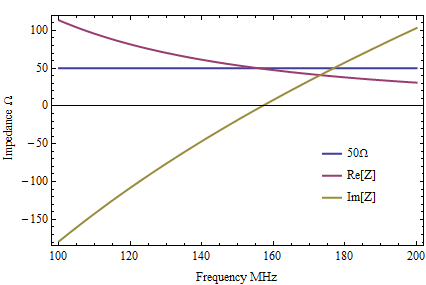
\includegraphics[width=100mm]{figures/Johnson_noise_thermometry/Impedance_matching2.png}
\caption{The real and imaginary impedance of an LC tank circuit (Eqn.~\ref{eq:LC_tank_Z}) with $R_0=1~k\Omega$, $C = 4.5~pF$, and $L = 220~nH$. The imaginary component cross zero as the real component is 50~$\Omega$.}
\label{fig:LC_tank_Z}
\end{figure}
Combining Eqn.~\ref{eq:LC_tank_Z} and Eqn.~\ref{eq:LC_tank_constraint} for a given $R_0$, $\omega_0$ and $Z_0$ gives us the needed inductance and capacitance values.
\begin{equation}\label{eq:LC_tank_LC}
L = \sqrt{\frac{R_0Z_0}{\omega_0^{~2}}}
\hspace{15mm}
C = \frac{1}{\sqrt{R_0Z_0\omega_0^{~2}}}
\end{equation}

While in theory adding a precise inductance and capacitance to a device is straight forward, in practice real devices can have a not insignificant amount of stray capacitance\footnote{stray inductance is also possible (particularly if long wire bonds are necessary) but are usually negligible for the resistance and frequency ranges in this thesis}. To account for this we can use a variable capacitor and tune the matching circuit to each device. One simple, temperature independent, magnetic field compatible capacitor that can be easily tuned is a set of twisted pair wires. Fig.~\ref{fig:picture_gimmicks} shows an example of a matching circuit using a twisted pair capacitor before and after tuning.
\begin{figure}
\centering
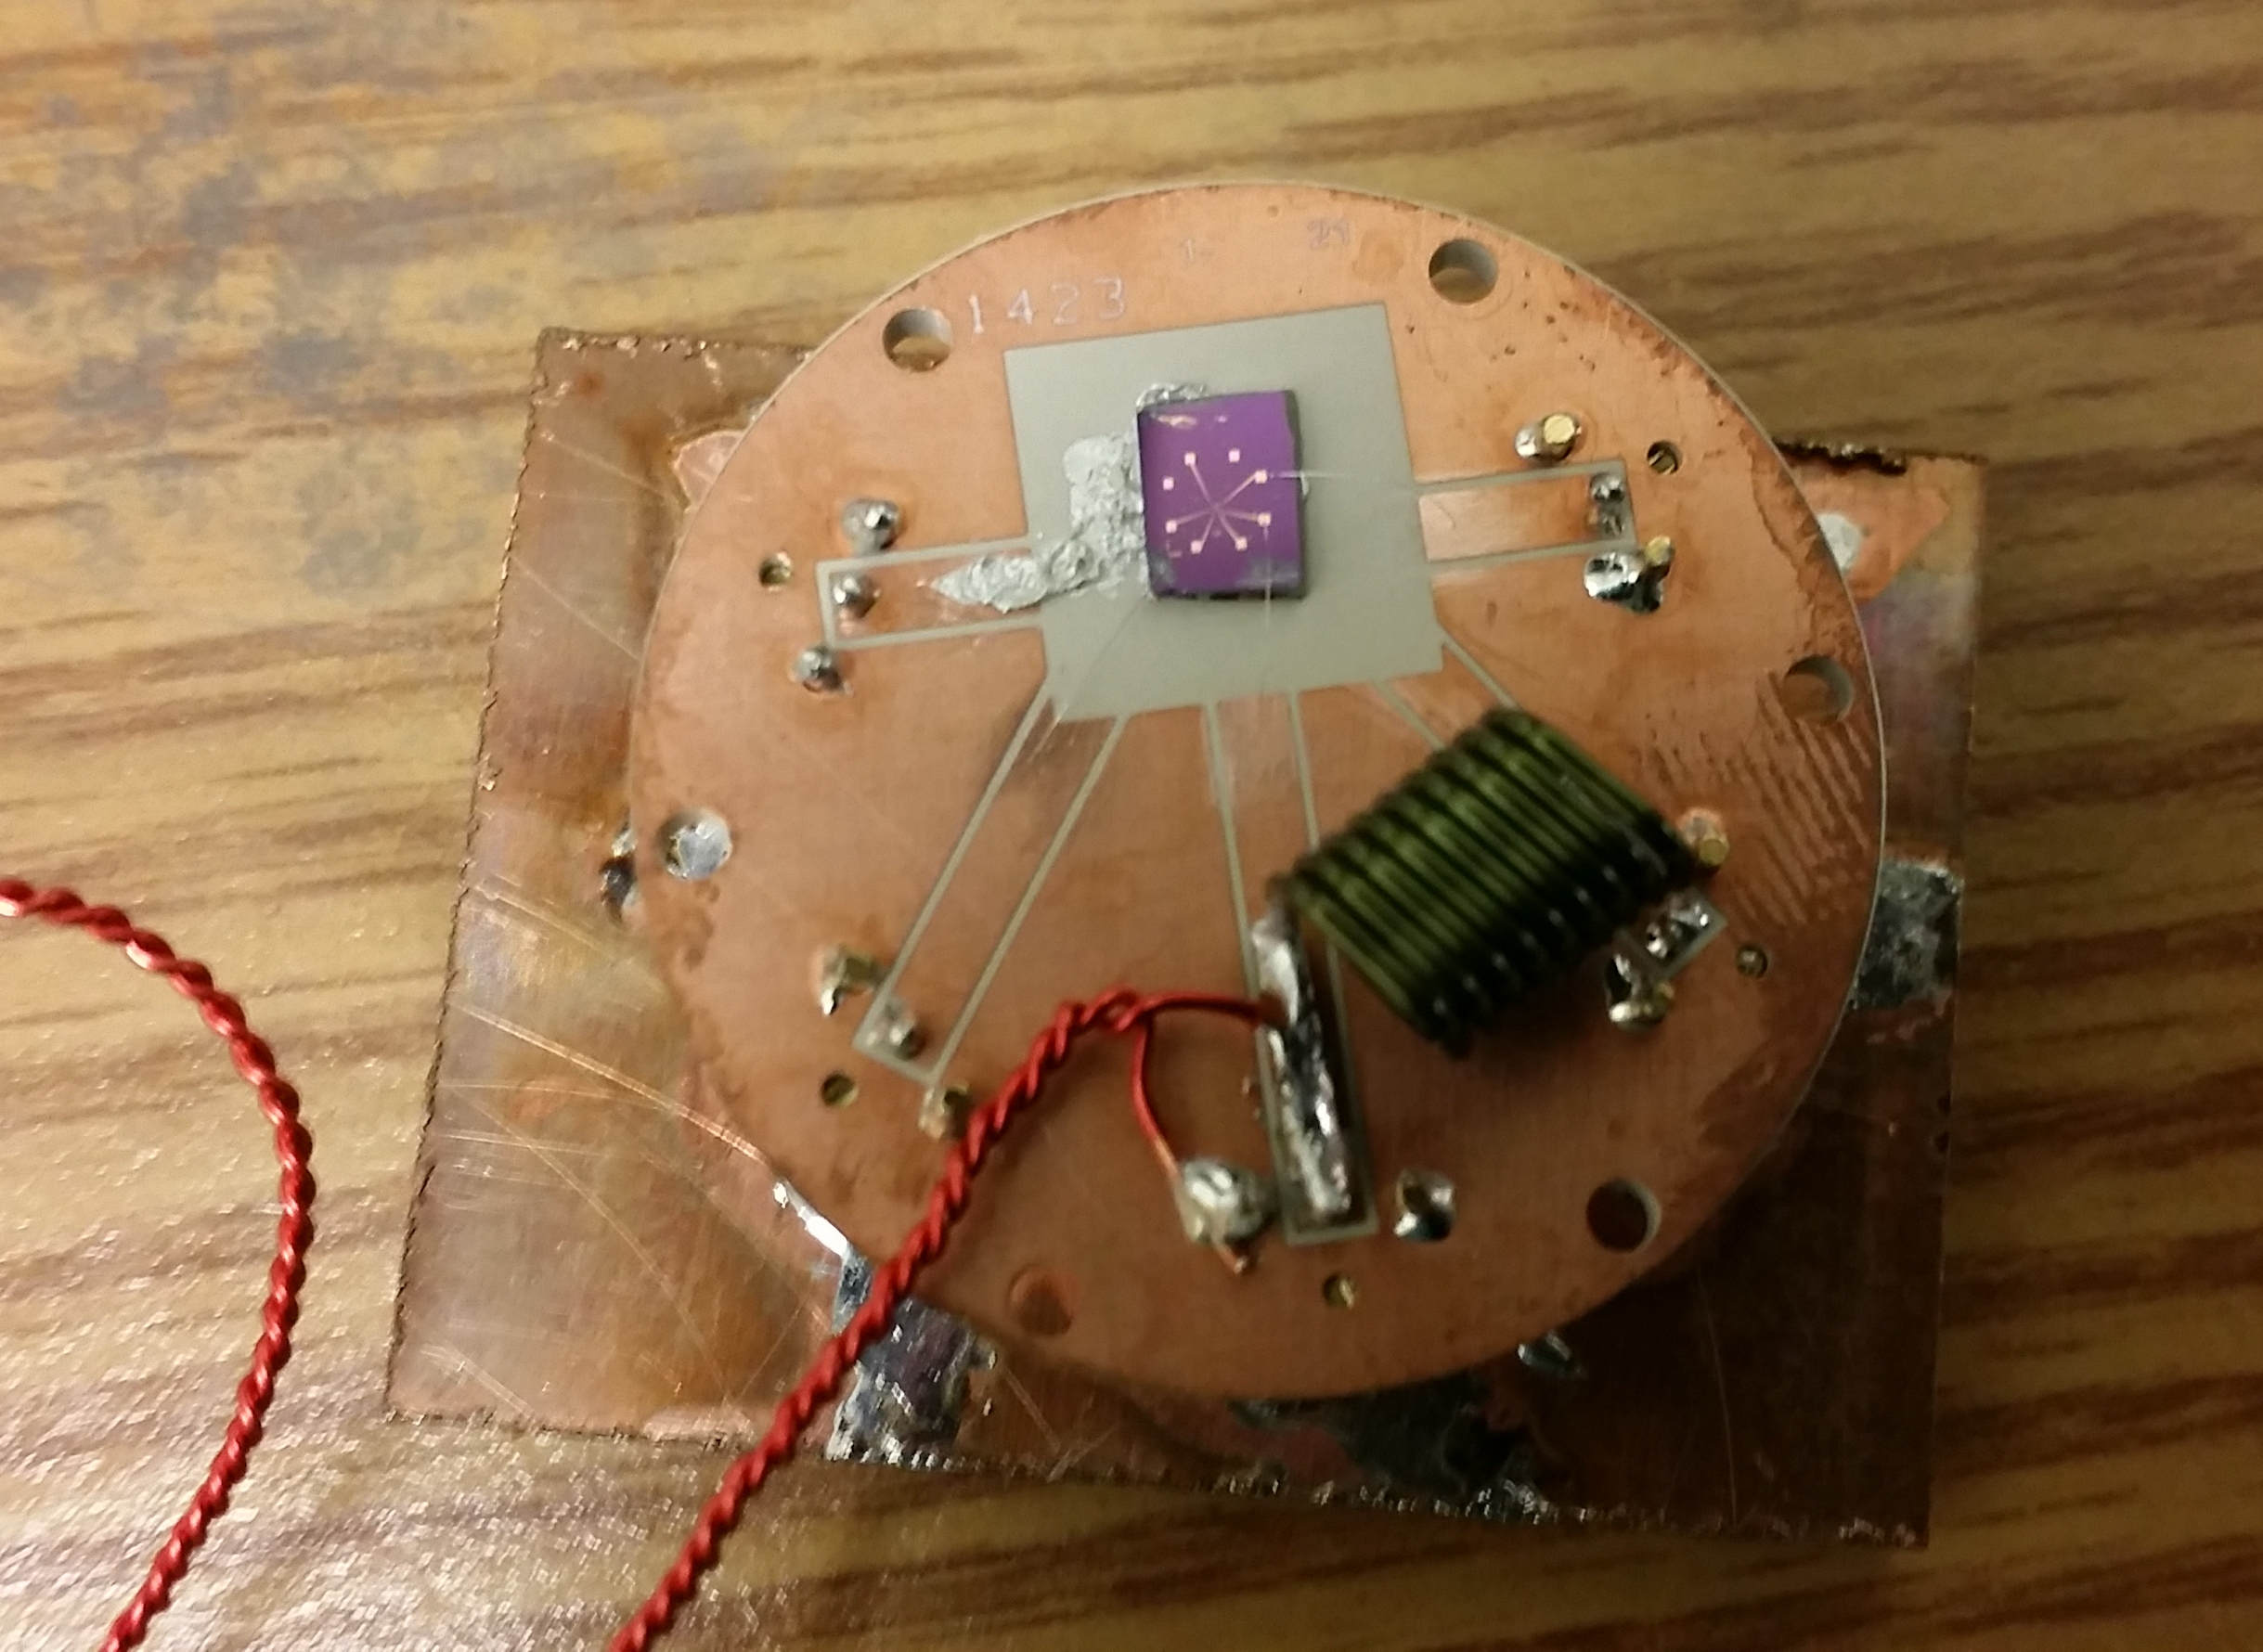
\includegraphics[width=0.5\textwidth]{figures/Johnson_noise_thermometry/picture_gimmick1.jpg}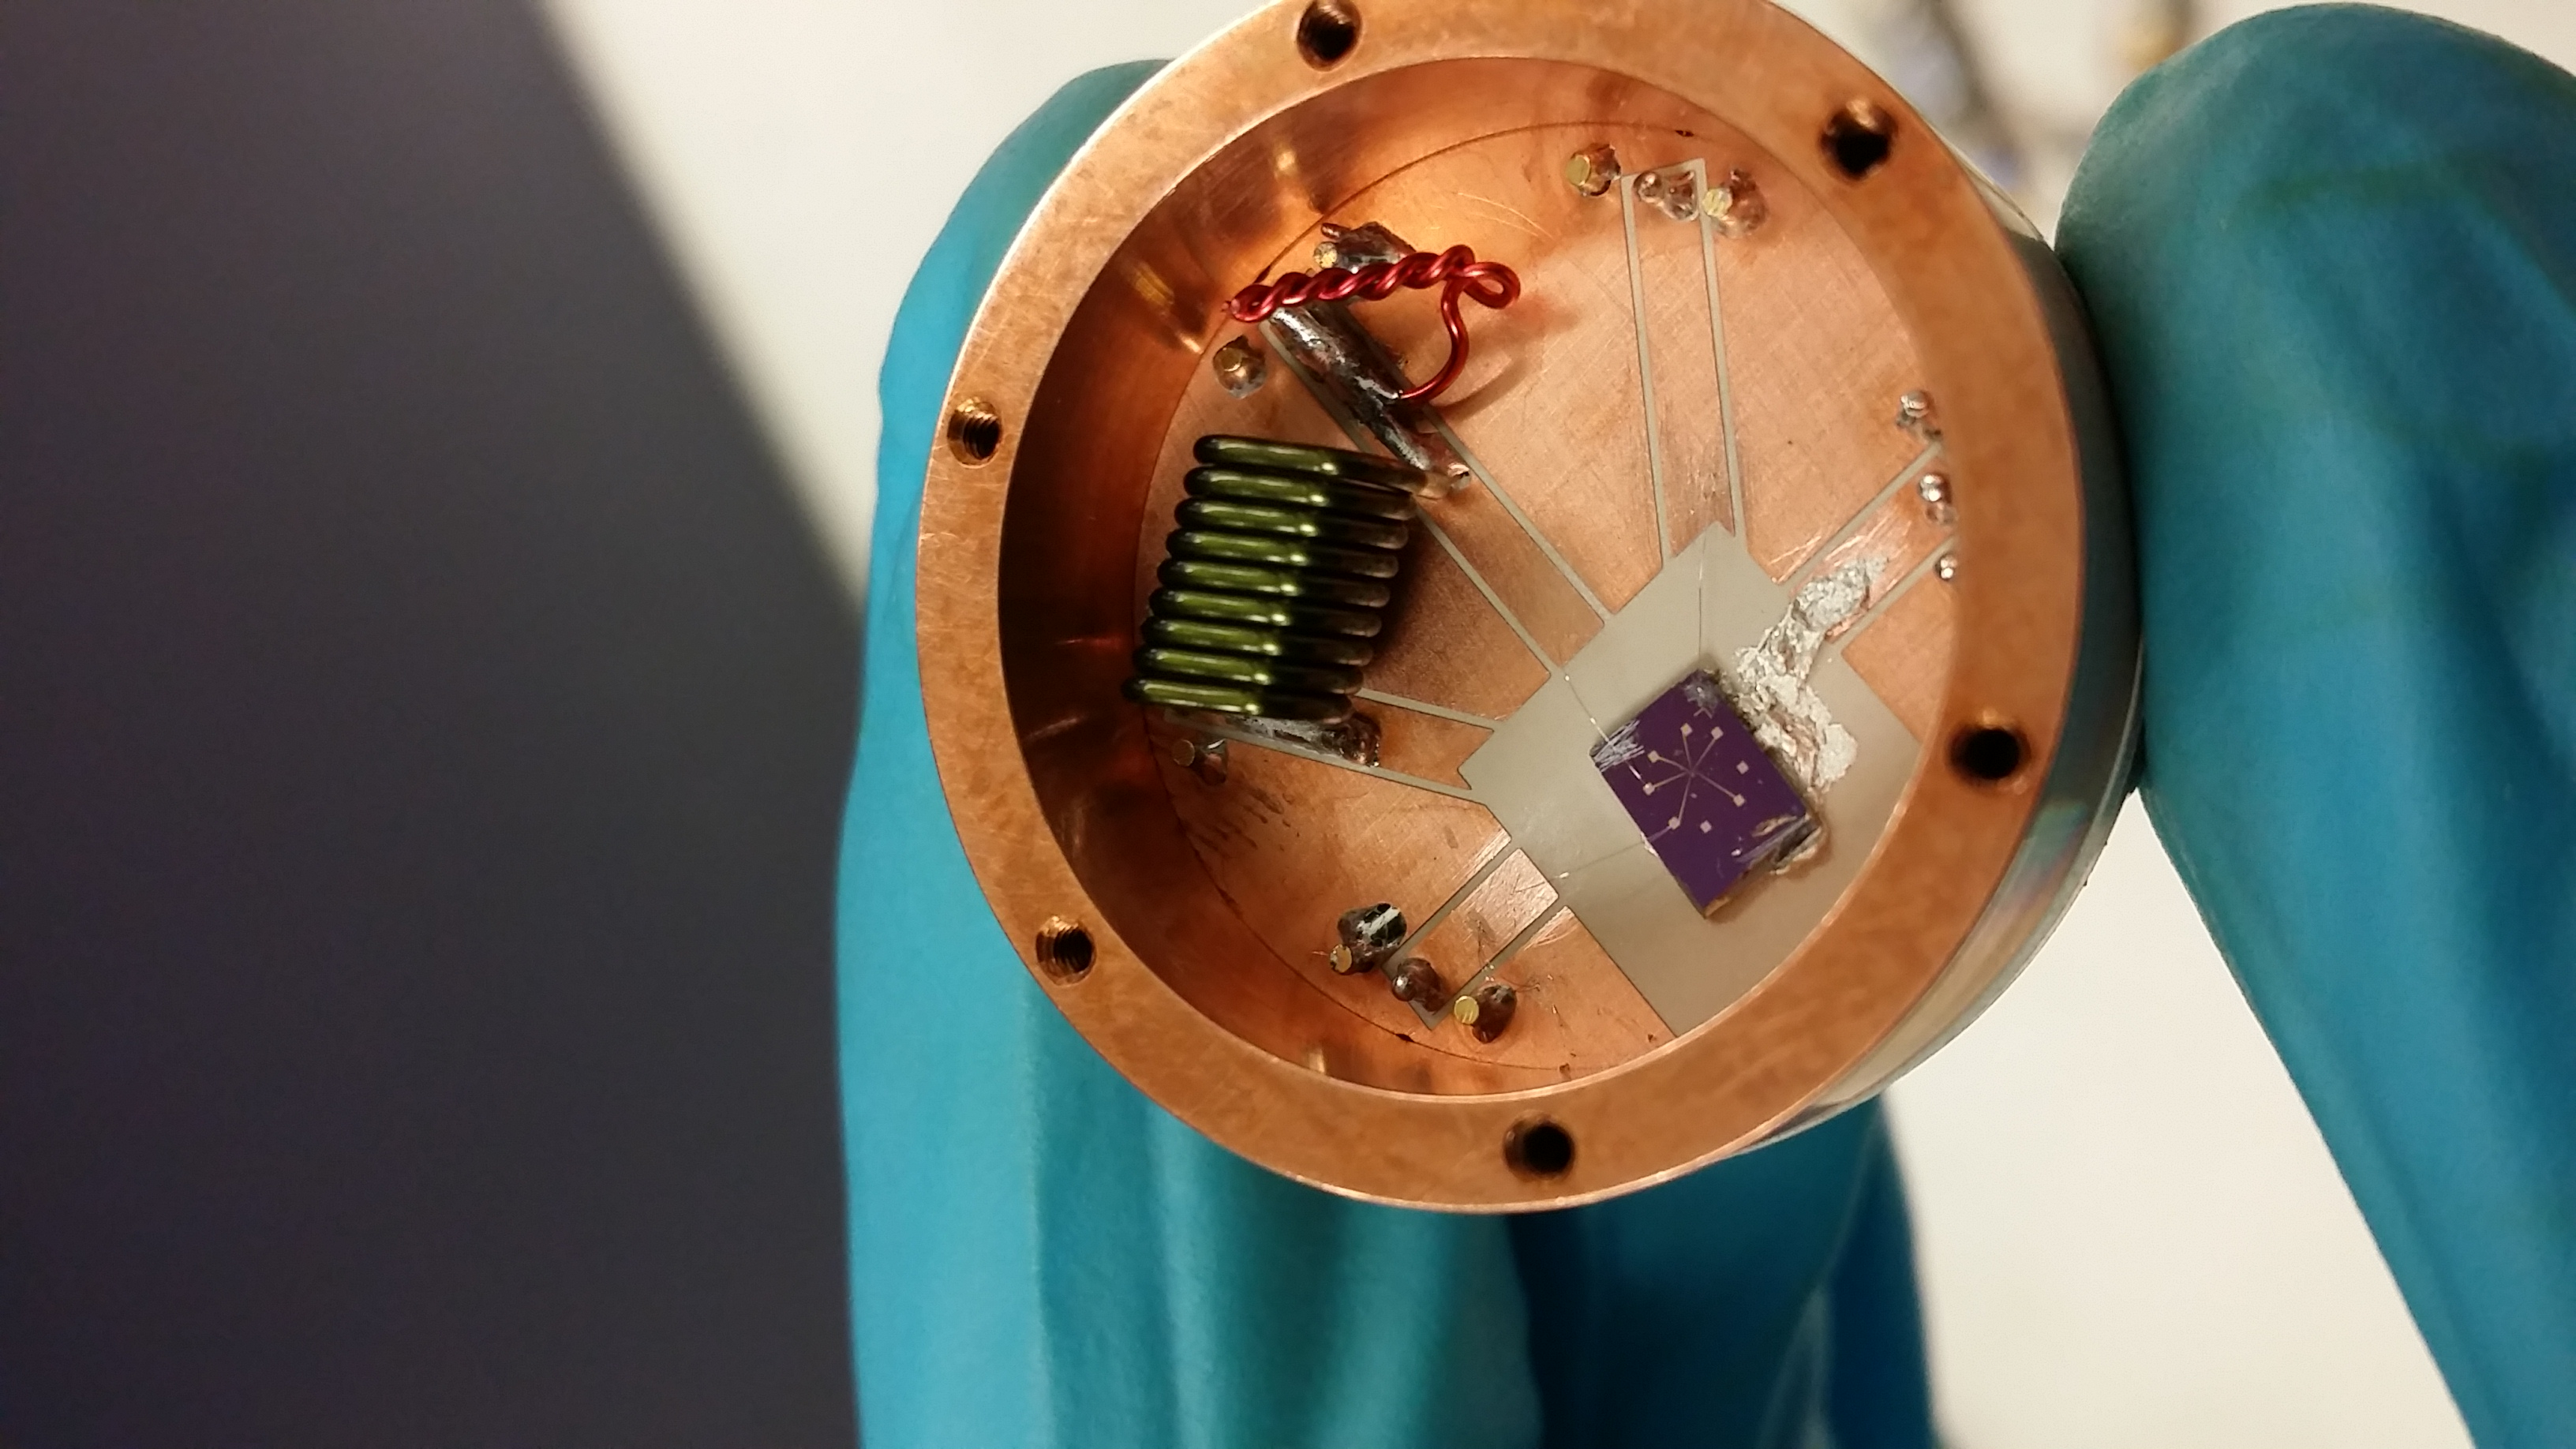
\includegraphics[width=0.5\textwidth]{figures/Johnson_noise_thermometry/picture_gimmick2.jpg}
\caption{Images of an impedance matching circuit before (\textbf{left}) and after (\textbf{right}) capacitance tuning. A long piece of twisted pair wire shunts the sample and an inductor (Coilcraft RF Air Core) is placed in series. To tune the capacitance, the twisted pair wire is cut shorter and shorter while the reflectance is monitored.}
\label{fig:picture_gimmicks}
\end{figure} 

A vector network analyzer (VNA) is used to measure the sample reflectance $\Gamma^2 = S_{11}^2$ to ensure the sample is properly matched. Fig.~\ref{fig:gimmick_tuning} shows how the reflectance changes for a $1~k\Omega$ sample impedance and $220~nH$ series inductance as the capacitance is tuned. When properly tuned we measure a large dip in $S_{11}^2$ signifying the sample is well coupled to the $50~\Omega$ VNA.
\begin{figure}
\centering
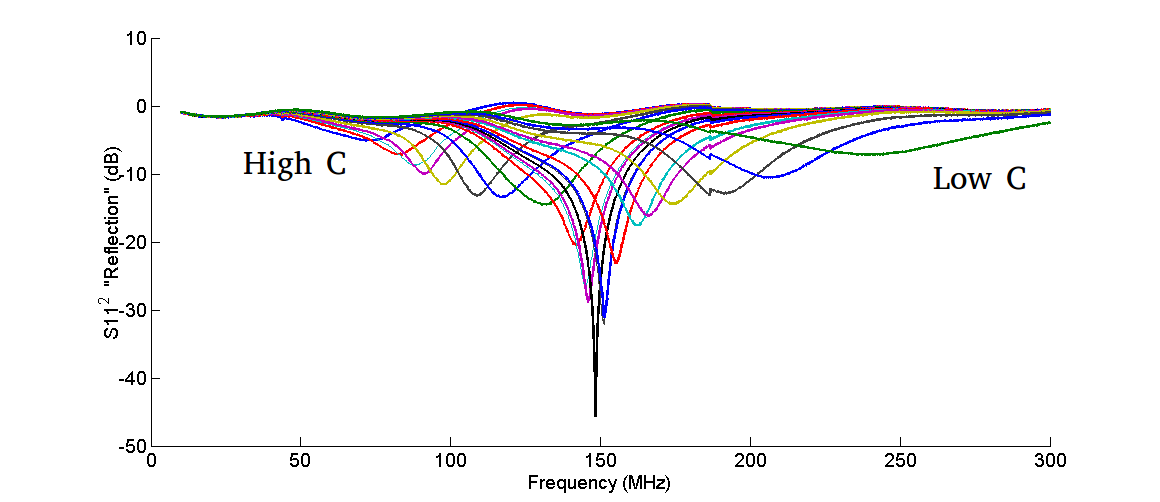
\includegraphics[width=\textwidth]{figures/Johnson_noise_thermometry/gimmick_tuning.png}
\caption{Reflectance curves while tuning a matching circuit for $R_0 = 1~k\Omega$ and $L = 200~nH$. The rightmost curve (green) corresponds to the lowest capacitance and the leftmost curve (blue) corresponds to the highest. Each curve is the result of cutting off a section of twisted pair wire.}
\label{fig:gimmick_tuning}
\end{figure} 

After matching, the noise spectral density emitted into the measurement circuitry is no longer flat but instead shaped by $\Gamma$ in accordance to Eqn.~\ref{eq:NyquistPower}. This point becomes clear when looking at the noise spectra emitted by an impedance matched sample at various temperatures --- as shown in Fig.~\ref{fig:spectrum_matching}; two features out prominently: first, the background noise is no longer flat but has structure and, second, the increase in noise as the sample temperature is raised is not the same at all frequencies. The result is that we are no longer free to select just any measurement bandwidth but must careful choose filters suited to the reflection profile.
\begin{figure}
\centering
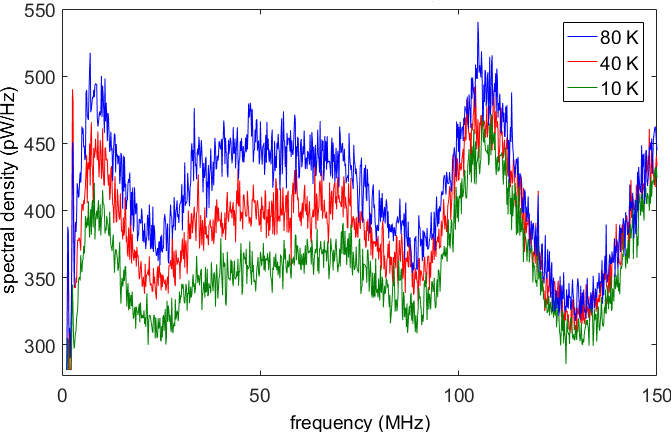
\includegraphics[width = 120mm]{figures/Johnson_noise_thermometry/Matched_spectra.png}
\caption{Amplified noise spectrum from a device, impedance matched using an LC tank circuit, at various temperatures. The background noise is no longer flat as the amplifier is not properly terminated at all frequencies. As the device temperature is raised, the spectral density increases non-uniformly as different frequencies couple differently to the circuitry as determined by Eqn.~\ref{eq:NyquistPower}}
\label{fig:spectrum_matching}
\end{figure}

In most mesoscopic measurements, the resistance of the device under test varies throughout the experiment; whether electrostatic gates modulate the carrier density, strong magnetic fields drive the system toward quantum hall, or cryogenic temperatures modify the conductivity, matching networks should operate over a wide dynamic range of input impedances. The response of a single stage LC matching network coupled to a variable resistance device\footnote{in this case a graphene device modulated via an electrostatic gate} is shown in Fig.~\ref{fig:S11vsR}. The device is optimally matched around $450~\Omega$ but maintains more than $10~dB$ coupling between $200~\Omega$ and $1~k\Omega$. As the resistance drops, we see the appearance of the trivial solution to Eqn.~\ref{eq:LC_tank_Z} of $R_0~=~50~\Omega$ and $\omega~=~0$. 
\begin{figure}
\centering
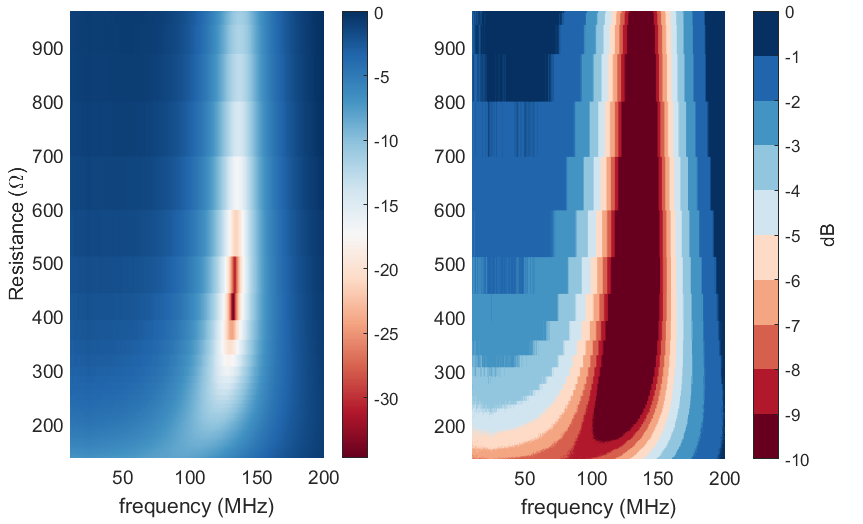
\includegraphics[width=120mm]{figures/Johnson_noise_thermometry/S11vsR.png}
\caption{Reflection coefficient $|S_{11}|^2$ for a single stage LC matching network as a function of device resistance. The left plot shows the full data set with a maximum coupling efficiency of more than $30~dB$. The right plot shows the same data with the color scale adjusted to highlight $1~dB$ changes up to a maximum of $10~dB$ (corresponding to $90\%$ coupling efficiency). All data taken from a graphene device at low temperature using an electrostatic gate.}
\label{fig:S11vsR}
\end{figure}

\subsection{Multi-stage matching}
Some experiments, such as the magneto-thermal transport studies discussed in chapter~\ref{ch:magneto-thermal_transport}, require devices to vary in resistance over multiple ordered of magnitude. Single stage LC networks are insufficient to cover this wide range. Fig.~\ref{fig:S11_3Rs} shows the loss of coupling in a single stage LC tank circuit at high device resistances. In this situation, multiple LC stages can be used to increase the dynamic range.
\begin{figure}
\centering
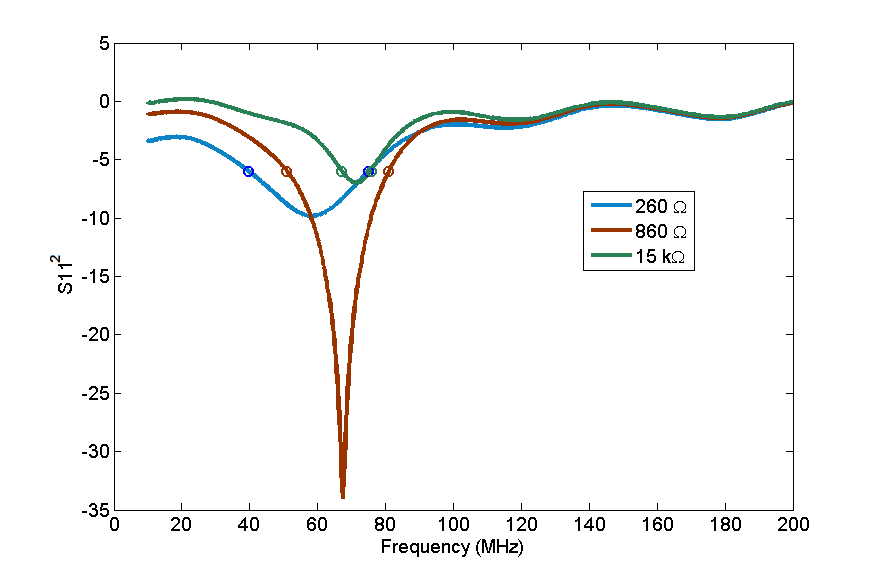
\includegraphics[width = 120mm]{figures/Johnson_noise_thermometry/S11_3Rs.png}
\caption{Reflection measurements of a single stage LC tank circuit coupled to a graphene device at different resistances. At high resistance the coupling drops off and reflection is high.}
\label{fig:S11_3Rs}
\end{figure}

Multi-stage LC networks allow you to match a wider area of the resistance-frequency space\footnote{This is a well known solution to a similar problem in audio recording. Multi-stage impedance transforms are used to capture the full audio range~\cite{horowitz_art_1989}.} by giving you multiple solutions to the equation $Z(\omega)=Z_0$. An example schematic of a two-stage LC tank circuit is shown in Fig.~\ref{fig:schematic_double_matching}. The resulting impedance takes the form:
\begin{equation}\label{eq:LC_double_tank_Z}
Z(\omega) = \left\lbrace\left[\left(R_0^{~-1}+i\omega C_1\right)^{-1}+i\omega L_1\right]^{~-1}+i\omega C_2\right\rbrace^{-1}+i\omega L_2
\end{equation}
\begin{figure}
\centering
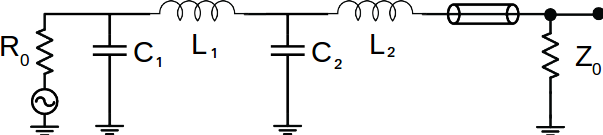
\includegraphics[width=100mm]{figures/Johnson_noise_thermometry/schematic_double_matching}
\caption{Schematic of a double-stage LC matching network. The device resistance $R_0$ to transformed to match the characteristic impedance of the measurement circuit $Z_0$ using two LC tank circuits. This results in a wider matching bandwidth and/or larger dynamic range depending on the values of the reactive elements.}
\label{fig:schematic_double_matching}
\end{figure}
Eqn.~\ref{eq:LC_double_tank_Z}, under the constraint defined by Eqn.~\ref{eq:LC_tank_constraint}, can have multiple solutions for the same set of inputs. This makes it possible to increase the matching bandwidth for the same dynamic range. Fig.~\ref{fig:LC_double_tank_Z} plots the real and imaginary components of Eqn.~\ref{eq:LC_double_tank_Z} for a specific choice of inductances and capacitances designed to cross $50+0i~\Omega$ at two nearby frequencies for the same device resistance. It can be shown for a fixed resistance that the maximum bandwidth occurs when the impedance is dropped by geometric factor~\cite{pozar_microwave_2011} --- i.e each stage transforms the impedance by the same factor. For an $N$ stage network of the form shown in Fig.~\ref{fig:schematic_double_matching}, the $i$th inductance and capacitance are given by a generalized form of Eqn.~\ref{eq:LC_tank_LC}. 
\begin{equation}\label{eq:LC_double_tank_LC}
L_i = \frac{\left(R_0^{~2N-2i+1}~Z_0^{~2i-1}\right)^{1/2N}}{\omega_0}
\hspace{15mm}
C_i = \frac{\left(R_0^{~2N-2i+1}~Z_0^{~2i-1}\right)^{-1/2N}}{\omega_0}
\end{equation}
\begin{figure}
\centering
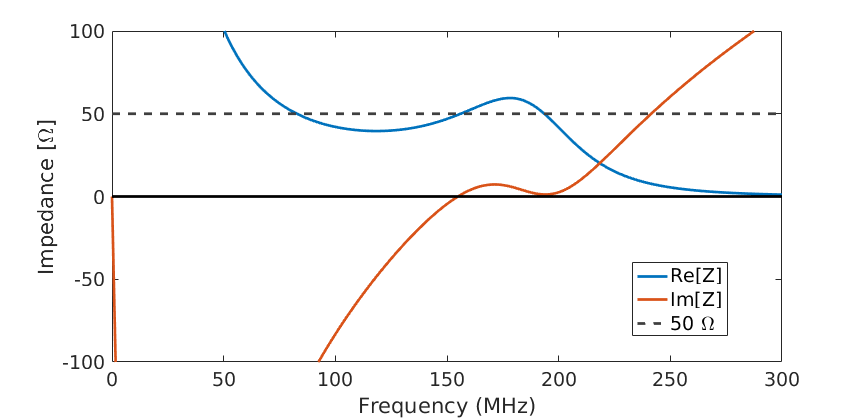
\includegraphics[width=120mm]{figures/Johnson_noise_thermometry/Z_doubleTank.png}
\caption{Real and imaginary components of Eqn.~\ref{eq:LC_double_tank_Z} for $R=1~k\Omega$, $C_1=1.9~pF$, $L_1=430~nH$, $C_2=8.6~pF$, and $L_2=96~nH$. The impedance goes to $50+0i~\Omega$ at two nearby frequencies.}
\label{fig:LC_double_tank_Z}
\end{figure}
Applying Eqn.~\ref{eq:LC_double_tank_LC} to a two-stage LC network with a graphene device we can increase the matched bandwidth to ${\sim}150~MHz$, as shown in Fig.~\ref{fig:S11vsR_double}.

However, if instead we want to match to larger range of resistances, we can move one of the solutions to Eqn.~\ref{eq:LC_double_tank_Z} to a higher resistance. This increases the dynamic range of the matching circuit at the expense of bandwidth. For example, by lowering the first capacitance of the network shown in Fig.~\ref{fig:S11vsR_double}, we move the high frequency solution from ${\sim}1~k\Omega$ to ${\sim}4~k\Omega$, increasing the dynamic range to include quantum hall resistances, as shown in Fig.~\ref{fig:S11vsR_double2}.
\begin{figure}
\centering
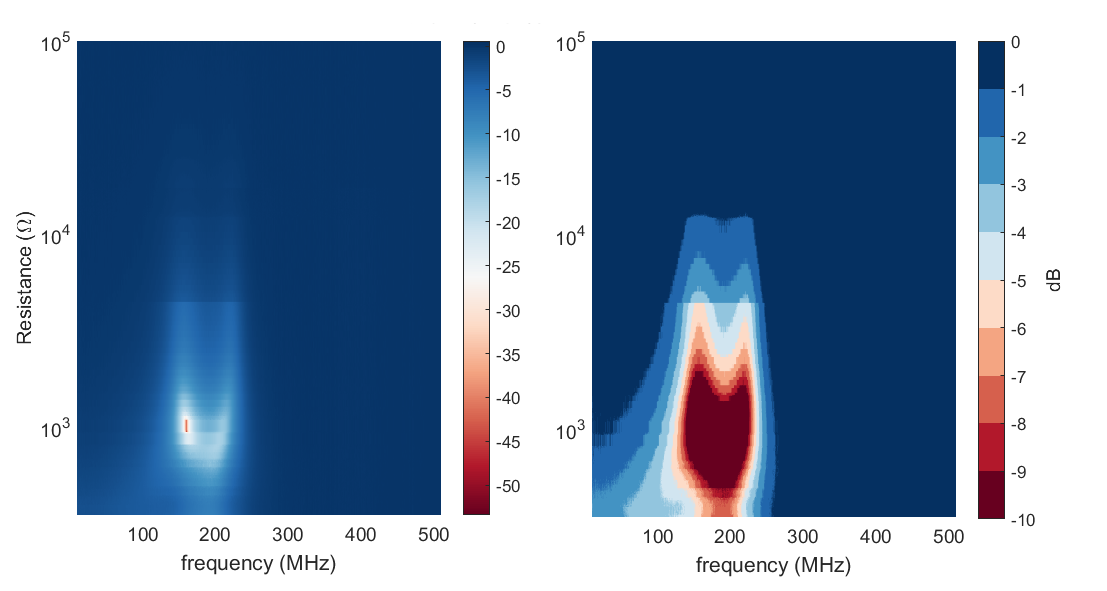
\includegraphics[width=\textwidth]{figures/Johnson_noise_thermometry/S11vsR_double.png}
\caption{Measured reflection coefficient |S11|$^2$ for a double stage LC matching network as a function of device resistance for reactive components following Eqn.~\ref{eq:LC_double_tank_LC}. The left plot shows the full data. The right plot shows the same data with the color scale adjusted to highlight 1~dB changes up to a maximum of 10~dB. The attached graphene device is optimally coupled at ${\sim}1~k\Omega$ and has an effective noise bandwidth of ${\sim}150~MHz$.}
\label{fig:S11vsR_double}
\end{figure}
\begin{figure}
\centering
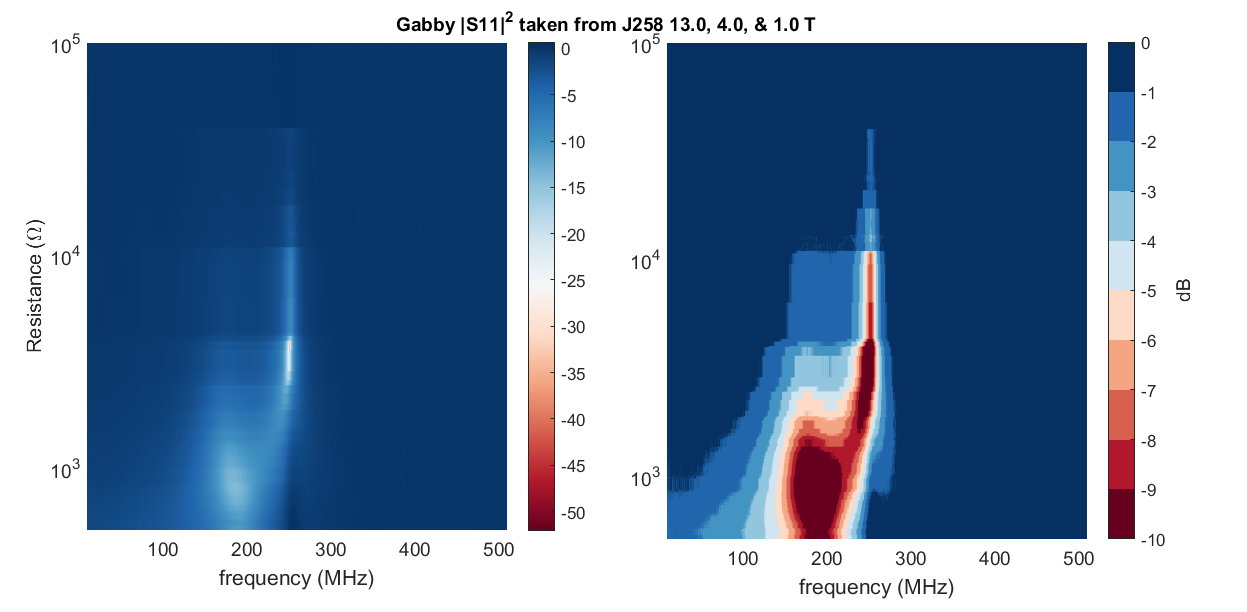
\includegraphics[width=\textwidth]{figures/Johnson_noise_thermometry/S11vsR_double2.png}
\caption{Measured reflection coefficient |S11|$^2$ for the same  double stage LC matching network shown in Fig.~\ref{fig:S11vsR_double} as a function of device resistance with the first stage capacitance lowered. This moves the high frequency solution to a higher resistance; effectively increasing the dynamic range at the cost of bandwidth. This technique enables the continuous measurement of graphene devices from zero field into the quantum Hall regime}
\label{fig:S11vsR_double2}
\end{figure}

The more stages added the wider the matched area in resistance-frequency space but also the more sensitive to stray capacitance the circuit becomes. In practice, devices with a $300~nm~SiO_2$ back-gate dielectric often have $3-6~pF$ stray capacitance; this can be reduced to less than $1~pf$ with the use of insulating substrates and local top-gates, or by increasing the back-gate dielectric to $1~\mu m$. Reducing the stray reactance also addressed the another challenge that comes with multiple matching stages --- it is no longer trivial to tune the circuit using gimmick\footnote{twisted pair wire is one form of a gimmick used to fine tune the circuit capacitance}. For these more complicated networks, surface mount ceramic capacitors can be soldered directly to the sample package, as shown in Fig.~\ref{fig:picture_doubleLC}, and adjustments can be made by careful removal and replacement\footnote{making sure to only apply heat locally to the capacitor to avoid damaging the sample.}.
\begin{figure}
\centering
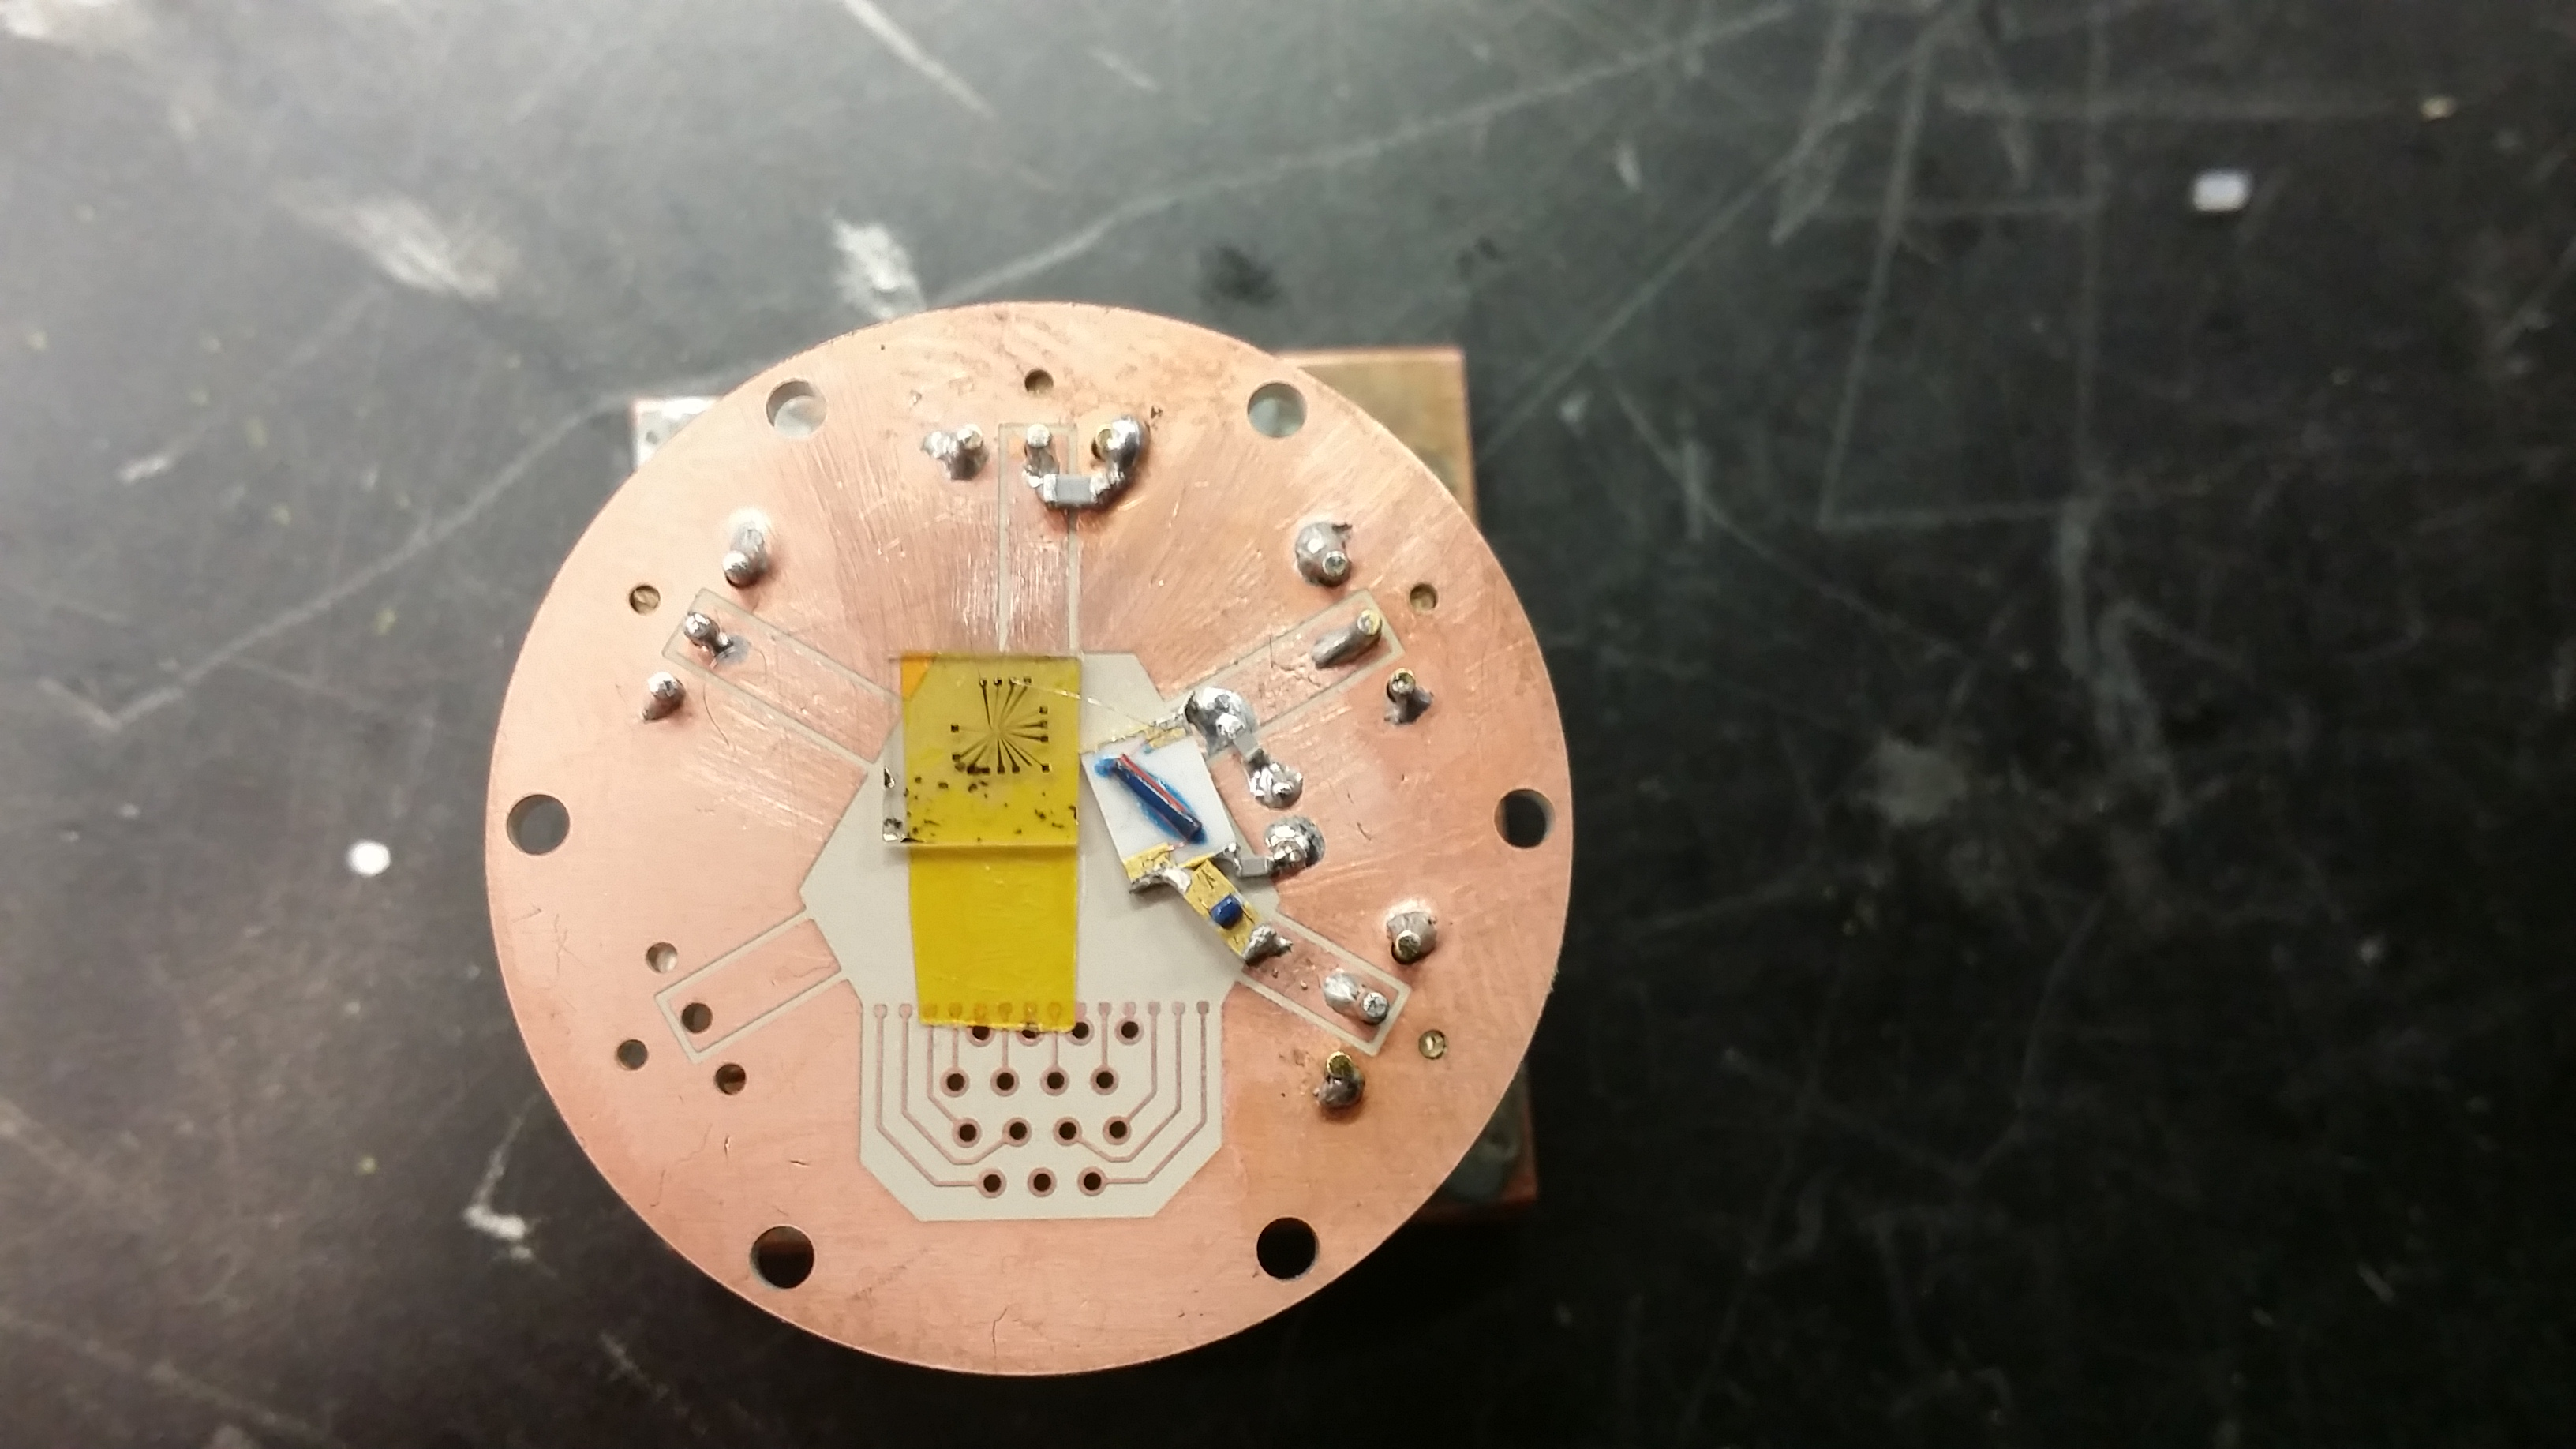
\includegraphics[width = 100mm]{figures/Johnson_noise_thermometry/picture_matching_ceramic}
\caption{Image of a two-stage LC matching network soldered directly to a custom cryogenic sample package and wire-bonded to a graphene device. Inductive elements have gold leads allowing direct wire-bonding. The sample is placed on an insulating sapphire substrate with a local top-gate to reduce the stray capacitance.}
\label{fig:picture_doubleLC}
\end{figure}

\section{System noise temperature}
\label{section:system_noise_temperature}
\newthought{A factor of two in signal to noise} can be the difference between graduating in two years or eight. From the Dicke radiometer formula, Eqn.~\ref{eq:dicke_formula}, the measurement time scales as the system noise temperature squared. Each component of the measurement circuit should be chosen with this in mind and, as such, its important to understand how each element affects the system as a whole.

The effective noise temperature, $T_n$, is the temperature at which your sample emits the same noise power as the sum of all the ``unwanted" noise in your system --- i.e. your signal to noise ratio is given by $T/T_n$, where $T$ is the sample temperature. Quantifying noise in this way lets us write the output voltage of our circuit, $V_{out}$, (which is proportional to the integrated noise power) as:
\begin{equation}\label{eq:power_output}
V_{out} = \mathcal{G}(\Gamma)(T+T_n(\Gamma))
\end{equation}
where $\Gamma^2$ is reflection coefficient between the sample and the amplifier and $\mathcal{G}$ is the generalized gain factor set by the LNA amplification together with the insertion loss of the microwave components integrated over the bandwidth defined by the external filters. In general, both $\mathcal{G}$ and $T_n$ are functions of $\Gamma$. All defining characteristics of a given given measurement circuit can be swept into $T_n$ and $\mathcal{G}$. In principle these factors must be measured but reasonable estimates can aid in the circuit design.

It is useful to distinguish the difference between the intrinsic noise temperature $T_0^n$ and the system noise temperature $T_n$. $T_0^n$ corresponds to the noise emitted by the circuit relative to the Johnson noise of a perfectly matched resistor, while $T_n$ is relative to the sample being measured --- i.e. $T_0^n$ can be reported on a device's specification sheet while $T_n$ is a function of the sample under test and can therefore change with experimental parameters such as electrostatic gate voltage and external field. In general $T_n$ is always equal to or greater than $T_0^n$

While $T_0^n$ is primary determined by the front-end amplifier, every component, $i$, with a finite intrinsic noise $T_i^n$ contributes an amount inversely proportional to the gain before that component, $G_i$. For example, if a circuit has three amplification stages with gains $G_1$, $G_2$, and $G_3$ with intrinsic noise temperatures $T_1^n$, $T_2^n$, and $T_3^n$, respectively, the total system intrinsic noise value is given by:
\begin{equation}
T_n^0 = T_1^n+\frac{T_2^n}{G_1}+\frac{T_3^n}{G_1G_2}
\end{equation}
or in general
\begin{equation}
T_n^0 = \sum_{i}\frac{T_i^n}{\prod_{j<i}G_j}
\end{equation}
Hence, if the front-end amplifier has a gain or $30~dB$, the noise from second amplifier is effectively reduced by a factor of $1,000$.

Estimating $T_n$ from $T_n^0$ requires knowing the matching function characterized by $\Gamma$. If $\Gamma$ is frequency independent then $T_n \approx T_n^0 / (1-\Gamma)$. For arbitrary $\Gamma(\omega)$ you can integrate over the bandwidth defined by external filters $\Delta f$\footnote{Eqn.~\ref{eq:Tn_integral} approximates the external filter function as a perfect square filter of bandwidth $\Delta f$. For the full calculation you must include the full filter function.}.
\begin{equation}\label{eq:Tn_integral}
T_n \approx \frac{1}{\Delta f}\ \int\limits_{\Delta f}\frac{T_n^0}{1-\Gamma(\omega)}d\omega
\end{equation}
\begin{figure}
\centering
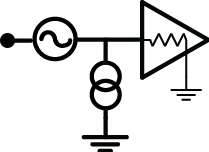
\includegraphics[width=40mm]{figures/Johnson_noise_thermometry/schematic_noise_IV.png}
\caption{schematic of a common noise model for active elements. A random voltage source is added in series with the signal and a random current source is added in parallel.}
\label{fig:schematic_noise_IV}
\end{figure}

The above formulation is approximate as it assumes the system's intrinsic noise can be described entirely by a single parameter $T_n^0$ --- a good assumption if the sample is properly matched. In general, active components require two parameters fully capture the noise behavior. A common technique is to model the circuit with an effective series voltage noise and parallel current noise, as shown in Fig.~\ref{fig:schematic_noise_IV}. However, an equivalent description, which is often more useful in microwave experiments, is that of a forward traveling noise power, $T_{n,for}^0$, a reverse traveling noise power $T_{n,rev}^0$, and some correlation between them. In the case of perfect matching, $\Gamma\rightarrow0$, $T_{n,rev}^0$ is completely absorbed. However for finite $\Gamma$ we can write the amplified noise as:
\begin{equation}\label{eq:P_full}
\langle P\rangle=G\ \left(T(1-\Gamma)+T_{n,rev}^0\Gamma+T_{n,for}^0\right)
\end{equation}
Rewriting this in the form of Eqn.~\ref{eq:power_output} and solving for $T_n$ and $\mathcal{G}$ yields.
\begin{equation}\label{eq:Tn_effective_full}
T_n(\Gamma)=\frac{\Gamma}{1-\Gamma}T_{n,rev}^0+\frac{1}{1-\Gamma}T_{n,for}^0
\end{equation}
and
\begin{equation}\label{eq:G_effective_full}
\mathcal{G}(\Gamma)=G(1-\Gamma)
\end{equation}

Eqn.~\ref{eq:Tn_effective_full} is what determines uncertainty, and therefore the speed of the measurement. An interesting side effect of Eqn.~\ref{eq:P_full} is that when the sample temperature is equal to $T_{n,rev}^0$, the total output noise has no dependence on $\Gamma$; no matter what resistance is being measured, the output noise power is the same! Fig.~\ref{fig:JNT_Vn_vs_R} shows the total noise power, Eqn.~\ref{eq:P_full}, as a function of sample resistance at several temperatures. The sample is optimally matche at ${\sim}10^3~\Omega$. In accordance with Eqn.\ref{eq:P_full}, at low sample temperature the noise decreases as $\Gamma$ decreases while at high temperature the noise increases as the sample approaches optimal matching. The spacing between curves is proportional to the generalized gain, $\mathcal{G}(\Gamma)$, which is maximized when $\Gamma$ is minimized.
\begin{figure}
\centering
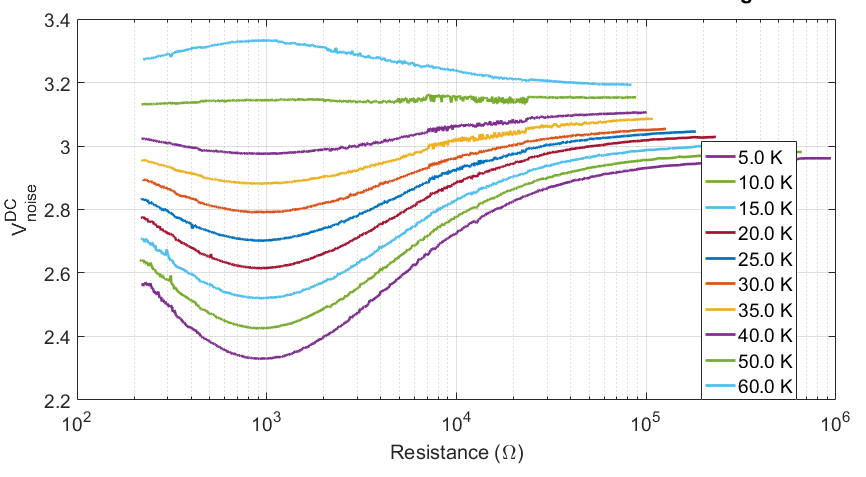
\includegraphics[width=120mm]{figures/Johnson_noise_thermometry/Vn_vs_R.png}
\caption{Voltage proportional to the total integrated noise power as a function of input sample resistance for different sample temperatures. The matching circuit is optimally matched ($\Gamma$ is minimized) at ${\sim}10^3~\Omega$. At low temperature, the total noise decreases as $\Gamma$ decreases, while at high temperature, the opposite is true. At $T\approx50~K$ the noise power is constant regardless of the input impedance in accordance with Eqn.\ref{eq:P_full} and $T_{n,rev}^0\approx50~K$.}
\label{fig:JNT_Vn_vs_R}
\end{figure}

\section{Calibration}
\label{section:calibration}
\newthought{Circuit losses and couplings are difficult to calculate a priori}, and while $T_n$ can be modulated away in a differential measurement, the generalize gain $\mathcal{G}(\Gamma)$ must be calibrated. If the output voltage is written in the form of Eqn.~\ref{eq:power_output} then $\mathcal{G}$ is given by:
\begin{equation}
\mathcal{G}(\Gamma) = \frac{dV_{out}}{dT}\bigg\rvert_{~\Gamma}
\end{equation}
The challenge here is fixing $\Gamma$. If the device under test has a fixed resistance then calibration can be done by recording $V_{out}$ for a few select bath temperatures. $\mathcal{G}$ is then given by the slope of a linear fit to $V_{out}(T)$. The inset of Fig.~\ref{fig:auto_noise_vs_T} shows $V_{out}(T)$ which was used to calibrate $\mathcal{G}$ yielding the main panel. However, most mesoscopic devices do not have a fixed resistance and thus more care must be taken in calibrating $\mathcal{G}(\Gamma)$.

The exact method of calibration will depend on the device characteristics and the size of the parameter space being measured. If the impedance of the device is sensitive to external parameters but only has a weak dependence on temperature --- i.e. $|dV_{out}/dT|$ is small and $V_{out}(T)$ is locally linear on a reasonable experimental scale --- then calibration can be done by taking local derivatives of $V_{out}(T)$ everywhere in the parameter space. While this method is straight forward to implement, it has several glaring drawbacks. Firstly, the time required to find local derivatives for the entire parameter space scales exponentially in the number of parameters. Secondly, it requires knowing the exact parameters that will be measured ahead of time; if during the course of an experiment the parameter space must be expanded or higher resolution is required, calibration must be done again.

A more robust method is to simultaneously measure both $V_{out}$ and $\Gamma$ and then numerically solve for $dV_{out}/dT$ for fixed $\Gamma$. Whats more, if the right reactive elements are used for impedance matching, $\Gamma$ becomes a function of only the resistance and fixing $\Gamma$ is equivalent to fixing $R$. Fig.~\ref{fig:JNT_Vn_vs_R} shows $V_{out}$ as a function of device resistance for various temperatures. It is important to note that each temperature curve is a collection of many different parameter sweeps that all collapse onto one smooth curve --- i.e. it does not matter if the sample is $13~k\Omega$ due to electrostatic gating at zero magnetic field, or due to the quantum Hall effect, the emitted noise is the same. If we attempt to fix external parameters and raise the temperature the output voltage is nonlinear, but if instead we fix the two-terminal resistance we arrive at Fig.~\ref{fig:JNT_Vn_vs_T}. Linear fits to each line then give $\mathcal{G}$ as the slope and $T_n$ as the offset\footnote{negative $T_n$ is where the linear fit intercepts the horizontal axis; also given by the offset divided by the slope}. For the data shown in Fig.~\ref{fig:JNT_Vn_vs_T}, the gain and noise temperature are shown in Fig.~\ref{fig:JNT_G_Tn_vs_R}; as expected the gain in maximized and the noise temperature is minimized at $R\sim 1~k\Omega$ where the sample is optimally matched. This particular data was taken from a two-stage matching network coupled to a graphene device and shows a dynamic range of ${\sim}3$ orders of magnitude in device resistance.
\begin{figure}
\centering
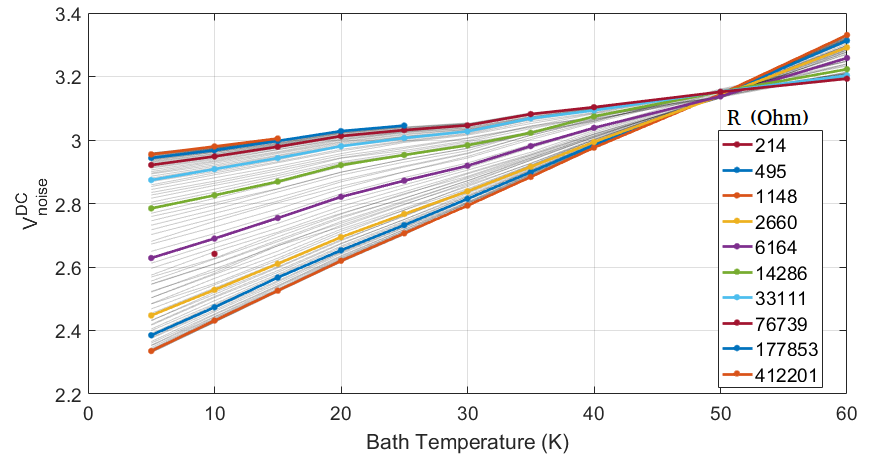
\includegraphics[width = 130mm]{figures/Johnson_noise_thermometry/Vn_vs_T}
\caption{Output voltage proportional to the integrated noise given by Eqn.~\ref{eq:power_output} as a function of device temperature with fixed resistance. The slope of each line gives the generalized gain $\mathcal{G}(R)$ while the extrapolated offset (divided by $\mathcal{G}$) is $T_n(R)$. The external parameters that result in a given resistance are generally different for different bath temperatures.}
\label{fig:JNT_Vn_vs_T}
\end{figure}
\begin{figure}
\centering
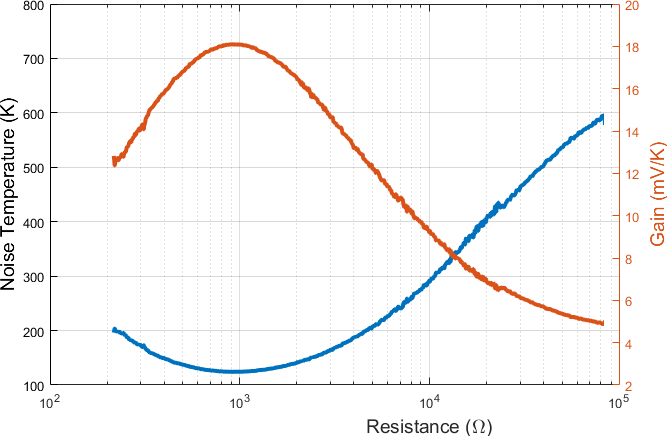
\includegraphics[width = 100mm]{figures/Johnson_noise_thermometry/G_Tn_vs_R}
\caption{Generalize gain and effective noise temperature exracted from data shown in Fig.~\ref{fig:JNT_Vn_vs_T}. The circuit is designed to optimally match an input resistance of ${\sim}1k\Omega$. As expected from Eqn.~\ref{eq:Tn_effective_full} and \ref{eq:G_effective_full}, the gain is maximized and the noise temperature is minimized when the device is effectively coupled --- i.e. $\Gamma$ is minimized. This two-stage LC tank circuit shows effective coupling over $3$ orders of magnitude of input resistance.}
\label{fig:JNT_G_Tn_vs_R}
\end{figure}


\section{Cross-correlated noise thermometry}

\newthought{A challenge in noise measurements} is isolating the noise you want to measure from the noise you don't. Dissipation between the resistive load and the LNA, such as coaxial attenuation and contact resistance, can contaminate thermal transport measurements~\cite{white_status_1996, glattli_noise_1997}. Johnson noise from the sample is added to the unwanted Johnson noise from these lossy components. Cross-correlation techniques can mitigate this problem by amplifying the Johnson noise signal of interest independently via two separate measurement lines~\cite{glattli_noise_1997, dicarlo_system_2006, henny_1/3-shot-noise_1999, brophy_correlatoramplifier_1965, klein_measurement_1979} and discarding uncorrelated noise between the two channels. The output voltage of such a scheme can be written as:
\begin{equation}
V_{out}\propto\langle\left(V_{JN}+V_{n1}\right)\times\left(V_{JN}+V_{n2}\right)\rangle 
\end{equation}
\begin{equation}\label{eq:crosscorrelation_expanded}
V_{out}\propto\langle V_{JN}^2\rangle + \langle V_{JN}V_{n1}\rangle+\langle V_{JN}V_{n2}\rangle+\langle V_{n1}V_{n2}\rangle
\end{equation}
where $V_{JN}$ is the instantaneous Johnson noise voltage and $V_{n1}$ and $V_{n2}$ are the instantaneous voltage noise on the two channels. If all noise sources are uncorrelated then only the first term in Eqn.~\ref{eq:crosscorrelation_expanded} is non zero and ${V_{out}\propto\langle V_{JN}^2\rangle}$
\begin{figure}
\centering
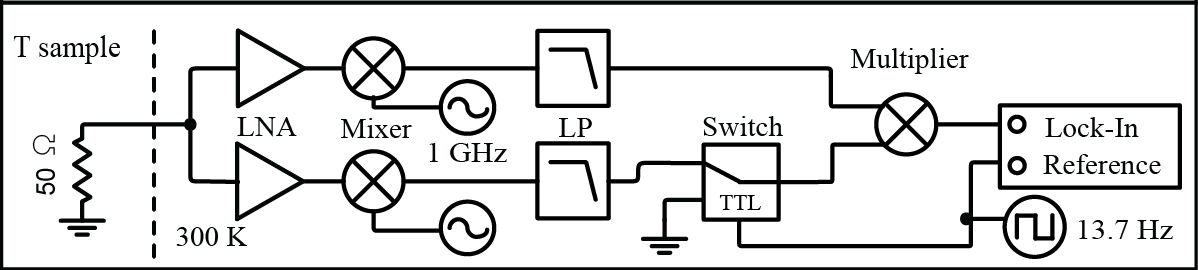
\includegraphics[width=\textwidth]{figures/Johnson_noise_thermometry/Schematic_Crosscorrelation.png}
\caption[JNT crosscorrelation schematic]{High level schematic of a typical Johnson noise thermometry cross-correlation measurement circuit. Noise from an impedance matched sample is sent into two independent measurement lines. Each line is then amplified, a measurement bandwidth is selected, and the signals are combined using a linear multiplier. A microwave switch acts as a chopper and the signal is integrated using a lock-in amplifier.}
\label{fig:schematic_crosscorrelation}
\end{figure}
Previously, cross-correlation measurements were limited to frequencies below a few MHz due to the practical implementation of multipliers and digital processing speeds~\cite{brophy_correlatoramplifier_1965, klein_measurement_1979, sampietro_high_2000, dicarlo_system_2006}. However, the $2~GHz$ analog multiplier (Analog Devices ADL5931) and LNA, combined with the lock-in amplifier modulation scheme described in Fig.~\ref{fig:schematic_crosscorrelation}, measure the correlated noise between the two channels, rejecting a large portion of the uncorrelated amplifier noise. The results are shown alongside an autocorrelation measurement (Fig.~\ref{fig:schematic_autocorrelation}) for comparison in Fig.~\ref{fig:cross_noise_vs_T}; the offset due to amplifier noise was reduced from $68~K$ to $2.6~K$.

\begin{figure}
\centering
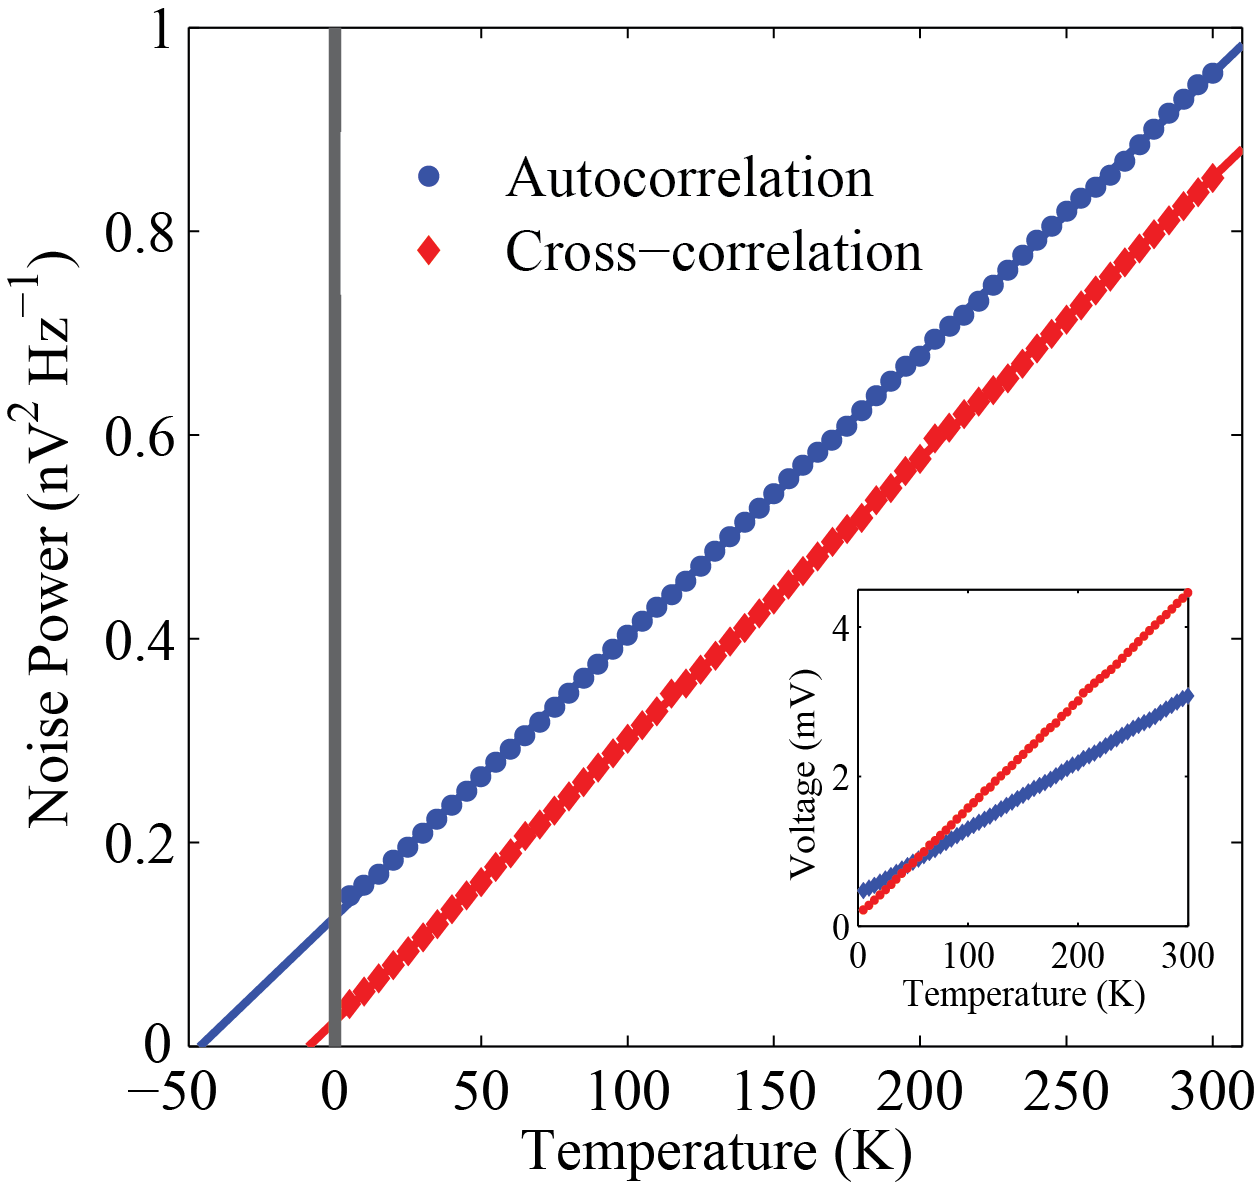
\includegraphics[width = 80mm]{figures/Johnson_noise_thermometry/Cross_noise_vs_T.png}
\caption{Auto- and cross-correlation Johnson noise measurements of a $50~\Omega$ resistor measured by the circuit shown in Figs.~\ref{fig:schematic_autocorrelation} and ~\ref{fig:schematic_crosscorrelation}, respectively. Inset shows the raw output voltage. The signal is converted to noise power by the Nyquist equation. The solid lines are linear fits, where the auto- and cross-correlation data exhibit an offset of $68~K$ and $2.6~K$, respectively, due to amplifier noise}
\label{fig:cross_noise_vs_T}
\end{figure}

Although the offset in the data is reduced by cross-correlation, the measurement time required to achieve a given precision is not reduced\footnote{Cross-correlation can improve the accuracy of an experiment but not the precision}. The time required to effectively average out the uncorrelated noise is still proportional to the amplifiers noise temperature. To be precise, $T_n$ is given by the geometric mean of individual amplifiers noise temperatures.
\begin{equation}\label{eq:cross_Tn}
T_n = \sqrt{T_{n1}T_{n2}}
\end{equation}
where $T_{n1}$ and $T_{n2}$ are the system noise temperatures of the two measurement lines. Using two LNAs with similar specifications Eqn.~\ref{eq:cross_Tn} reduces to the Dicke formula, Eqn.~\ref{eq:dicke_formula}. Fig.~\ref{fig:cross_sensitivity} illustrates this point by showing the standard deviation of $1000$ temperature measurements as a function of integration time. Both auto- and cross-correlation measurements follow the Dicke formula with similar magnitude and uncertainty scaling as $\sqrt{\tau}$ and $\sqrt{\Delta f}$.
\begin{figure}
\centering
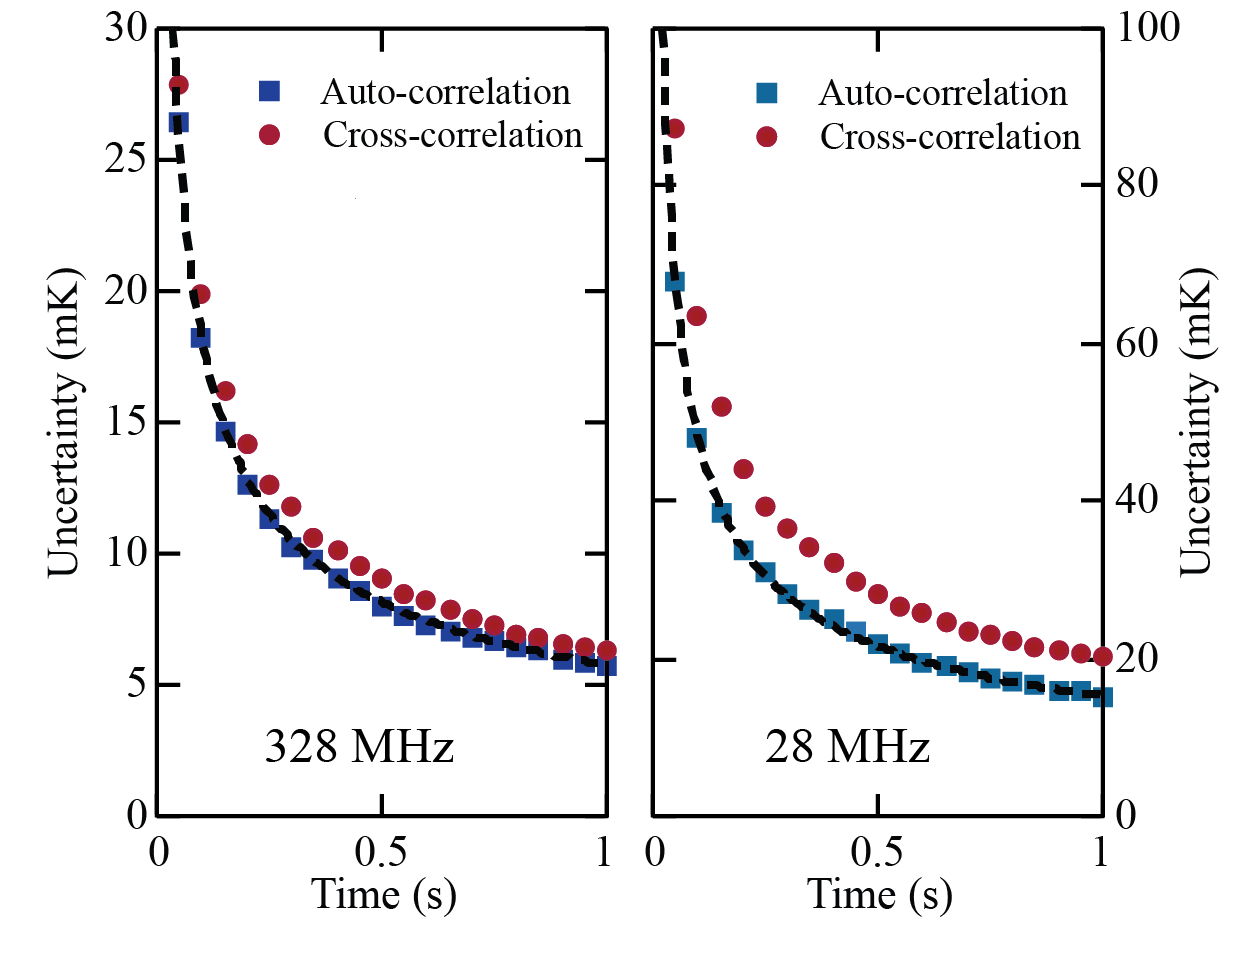
\includegraphics[width = 100mm]{figures/Johnson_noise_thermometry/cross_sensitivity.png}
\caption{Standard deviation of $1000$ auto- and cross-correlation temperature measurements as a function of integration time for $328~MHz$ (left) and $28~MHz$ (right). In all cases, uncertainty follows the Dicke relation, Eqn.~\ref{eq:dicke_formula}, scaling as $\sqrt{\tau}$ and $\sqrt{\Delta f}$. Data is taken from a $50~\Omega$ resistor}
\label{fig:cross_sensitivity}
\end{figure}
 

\subsection{multi-terminal cross-correlation}
Cross-correlation can be used to reduce the effects of contact and lead resistance with the use of multi-terminal devices. However, as discussed in section~\ref{section:TJN}, the voltage fluctuations on different pairs of terminals can measure different areas of a device. For example, the four-terminal device drawn in Fig.~\ref{fig:4terminal} will give very different results depending on which terminal are paired --- cross-correlation between $V_{AD}$ and $V_{BC}$ will by more sensitive to the device temperature than cross-correlation of $V_{AB}$ and $V_{CD}$. The exactly amount of overlap between between the noise on any pair of terminals can be found via the method described in section~\ref{section:TJN}.
\begin{figure}
\centering
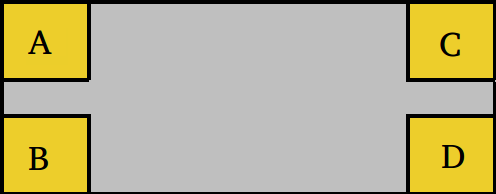
\includegraphics[width=80mm]{figures/Johnson_noise_thermometry/4terminal.png}
\caption{Cartoon of a four-terminal device. If the voltage between terminals A and D is cross-correlated to the voltage between terminals B and C, the result will be more sensitive to the temperature of the device than pairing A-B and C-D}
\label{fig:4terminal}
\end{figure}

